\section{Technical Implementation}
\label{section:techimpl}
This section describes the current solution, the implemented software architecture and the final results of the project.

\subsection{System Overview}
The following graphics displays the current system overview.
As described in \sectionref{section:techimpl:arcgis} and \sectionref{section:project:swisstoporeplacement}, instead of the elevation model data from \emph{swisstopo}, a Unity plugin for \emph{ArcGIS} maps services was used.
This change is reflected in the new system overview, and is the only adjustment that was made.

\begin{figure}[H]
    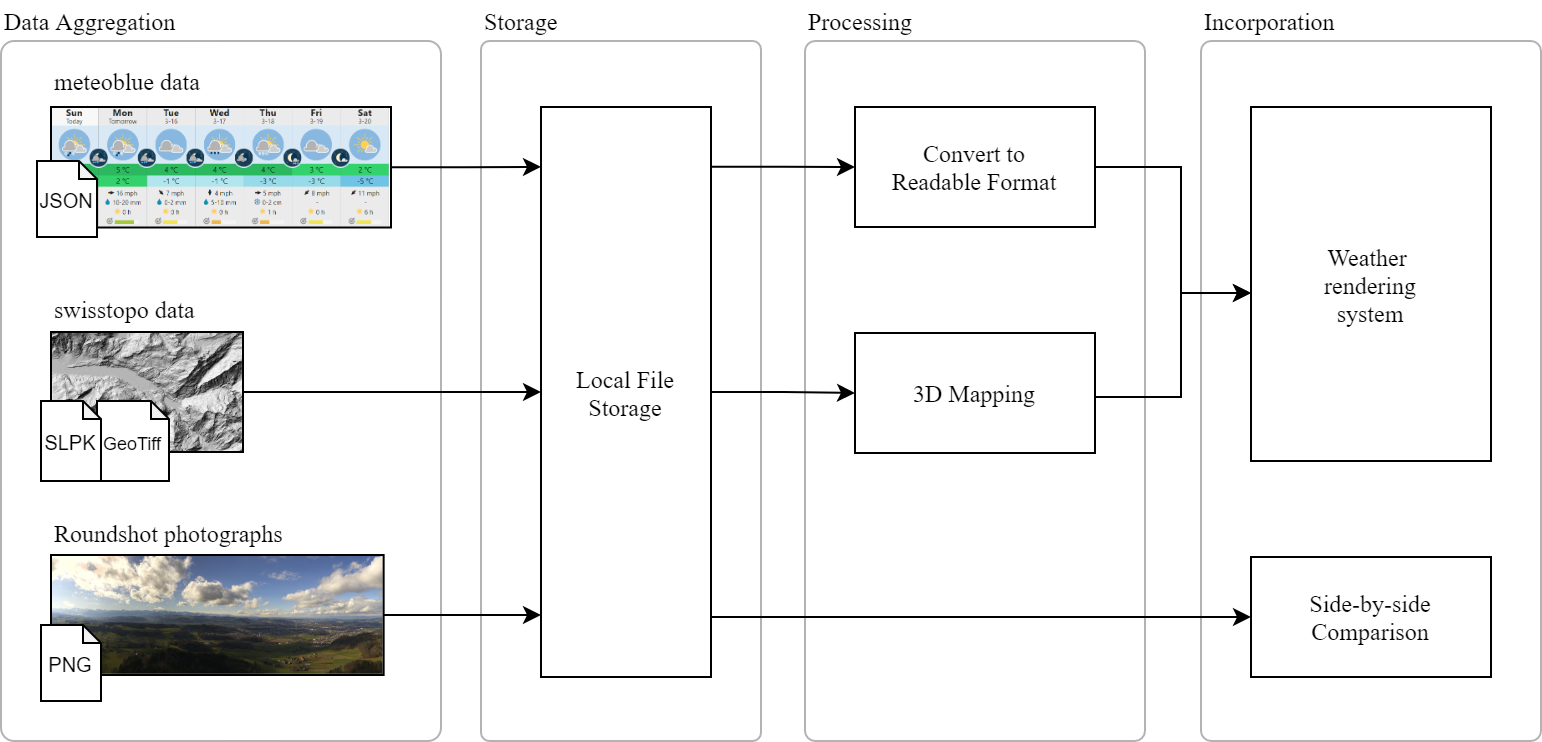
\includegraphics[width=\linewidth]{system diagram.png}
    \caption{The system overview diagram.}
    \label{img:techimpl:system}
\end{figure}

\clearpage

\subsection{Meteoblue Integration}
\label{section:techimpl:meteoblue}
While the bachelor project specifictation document described the use of \emph{meteoblue}'s "basic 1h" package, this was not the only package that was used in the final implementation.
After the cancellation of the technical interview with \emph{meteoblue} and further research into additional, available weather data sources, the package "clouds 1h" was suggested.
It provides an overview of cloud coverage percentage for each cloud layer, which is exactly what the implementation was missing.
\emptyline
\begin{tabularx}{\linewidth}{|l|X|}
    \hline
    \textbf{Package name}   & \textbf{Description} \\ \hline
    Basic (1h)              & Mainly used for shading and visual effects. \\ \hline
    Clouds (1h)             & Mainly used for cloud coverage data. \\ \hline
\end{tabularx}
\emptyline
The following table displays a list of properties from both data packages and how they are used in the final implementation.
\emptyline
\begin{tabularx}{\linewidth}{|l|l|X|}
    \hline
    \textbf{Property name}      & \textbf{Source}     & \textbf{Usage}                                 \\ \hline
    Wind speed                  & Basic (1h)          & Used with a multiplier                         \\ \hline
    Wind direction              & Basic (1h)          & Converted form degrees to a directional vector \\ \hline
    Precipitation               & Basic (1h)          & Used for controlling rain particle system and cloud color.\newline Factored into cloud edge highlight colors from sunshine.\newline Factored into skybox colors. \\ \hline
    Precipitation probability   & Basic (1h)          & Included in approximation of precipitation     \\ \hline
    Cloud coverage low          & Clouds (1h)         & Used for the weather in Bern                   \\ \hline
    Cloud coverage mid          & Clouds (1h)         & Used for the weather in Bern                   \\ \hline
    Cloud coverage high         & Clouds (1h)         & Used for the weather in Bern                   \\ \hline
    Total cloud coverage        & Clouds (1h)         & Used for the distant weather                   \\ \hline
\end{tabularx}
\emptyline
Other properties like temperature and UV index provide insufficient or irrelevant information and have therefore not been mapped.

\subsection{ArcGIS Integration}
\label{section:techimpl:arcgis}
During the research phase of the project, the \emph{ArcGIS Maps SDK for Unity} \cite{arcgis:unitysdk} was found. This proved to be a suitable replacement for the originally planned \emph{swisstopo} elevation model data.
The plugin was easily installed. The setup process required minimal amount of effort and the plugin was ready to run in no time. 

\begin{figure}[H]
    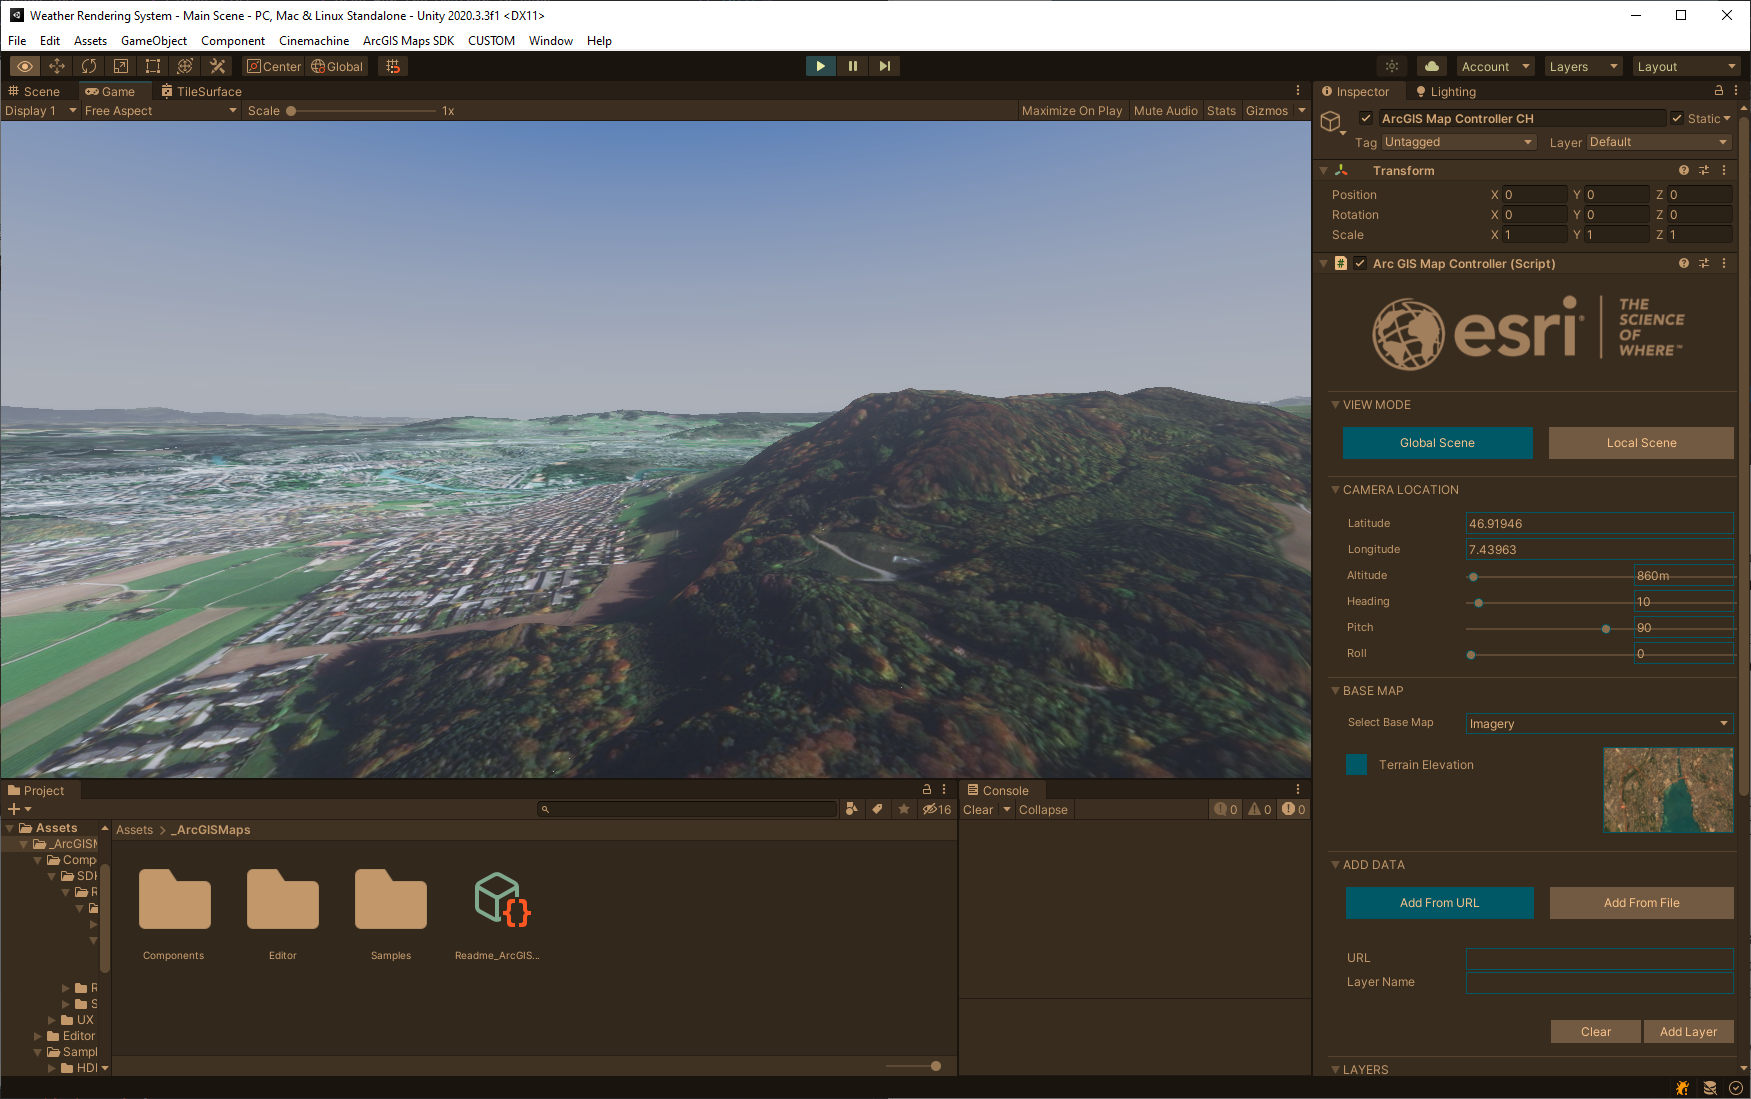
\includegraphics[width=\linewidth]{unity-sdk2.png}
    \caption{ArcGIS Maps SDK for Unity \protect\cite{arcgis:unitysdk}.}
\end{figure}

\noindent
The plugin generates and renders map tiles according to the elevation model and automatically maps aerial photographs as textures on top.
This happens during runtime and is continuously updated.
\\
After setting up the plugin in Unity, the camera needed to be positioned on top of the Gurten mountain. Also, there needed to be a translation mechanic to move the camera to the top of the Bantiger mountain.
This was done with via script and is not part of the \emph{ArcGIS} plugin.

\subsection{Unity Project Architecture}
\begin{wrapfigure}[13]{r}{4cm}
    \vspace{-\baselineskip}
    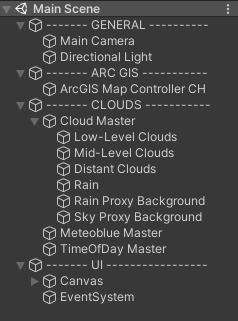
\includegraphics[width=4cm]{unity scene hierarchy.png}
    \caption{Hierarchy of the Unity project.}
    \label{img:techimpl:hierarchy}
\end{wrapfigure}
The project architecture in Unity consists of a set of \gls{volumetric} \gls{shader}s, the \emph{ArcGIS} component and some auxiliary objects.
\\
\autoref{img:techimpl:hierarchy} shows the content of the Unity scene file.
The first section, named "general", contains the standard game objects for the primary camera and for the directional lighting.
\\
The \emph{ArcGIS} component only requires a single game object, which has been placed into its own section.
\\
It is followed by the core of the weather rendering system, which is housed under the section named "clouds".
In it, there are several controlling game objects like the "meteoblue master", which are responsible for setting up the shaders.
\\
At last, the "UI" section contains the default game objects for a \gls{ui} in Unity, adjusted to this project.

\clearpage

\subsubsection{Scene Anatomy}
The scene setup is similar to what was originally planned in \sectionref{section:impl:layers}. There are multiple layers of clouds, each rendered by a unique \gls{volumetric} \gls{shader}.
However, there is no layer for high-level clouds. It turned out that the intricate visual appearance of cirrus clouds was more difficult to simulate than anticipated.
Also, there is no dedicated layer for ground fog, as the Unity engine already offers a way to include fog into the scene.
\\
The current scene anatomy is depicted in the following graphic, as viewed from the side.

\begin{figure}[H]
    \centering
    \begin{tikzpicture}[scale=1]
        \tikzset{edge/.style = {-{Latex[length=3mm]},shorten >= -4pt}}
        \tikzset{shortedge/.style = {shorten <=-4pt,shorten >= -4pt}}
        \tikzset{icon/.style = {font=\Large}}
        \tikzset{mini/.style = {font=\footnotesize}}
        \tikzset{tiny/.style = {font=\tiny}}

        % cloud layer boxes
        \node[inner sep=0pt] at (6,4) 
            {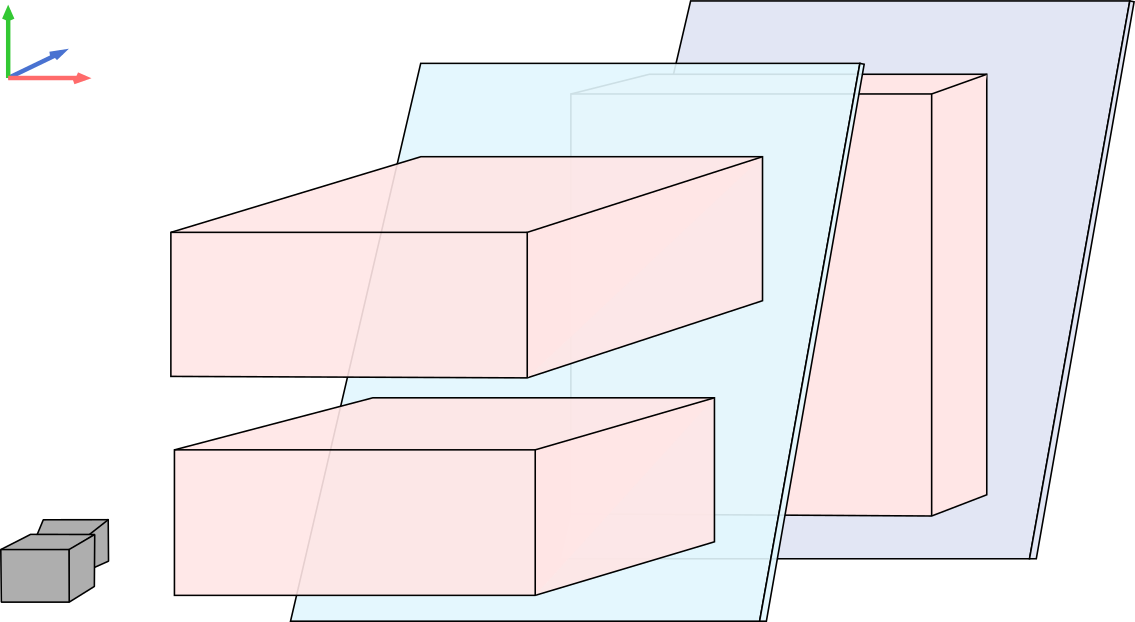
\includegraphics[width=0.8\textwidth]{anatomy.png}};

        \node at (0.3,0.4) {camera};

        % labels
        \node[red] at (2.3,2.1) {$C_{low}$};
        \node[red] at (2.3,4.5) {$C_{mid}$};
        \node[red] at (9.65,2.6) {$C_{back}$};
        \node[darkercyan] at (4.60,6.42) {$P_{rain}$};
        \node[darkercyan] at (7.50,7.10) {$P_{sky}$};
        \node[tiny] at (00.95,6.52) {$x$};
        \node[tiny] at (-0.06,7.45) {$y$};
        \node[tiny] at (00.66,6.91) {$z$};
        
    \end{tikzpicture}
    \captionof{figure}{Final Unity scene anatomy.}
    \label{img:tikz:techimpl:anatomy}
\end{figure}

\noindent
In the scene, there are three cloud layers: \color{red}$C_{low}$\color{black}, \color{red}$C_{mid}$ \color{black} and \color{red}$C_{back}$\color{black}.
The \gls{shader} for layer \color{red}$C_{low}$ \color{black} handles low-level clouds like the puffy cumulus, while \color{red}$C_{mid}$ \color{black} is responsible for rendering mid-level clouds of the "alto"-type.
Both front layers use weather data for Bern, Switzerland.
Behind the two front layers, there is \color{red}$C_{back}$\color{black}, which renders an approximation of cumulonimbus clouds. It uses the weather data of the correspondent location in the distance (either Solothurn or Fribourg) instead of Bern.
\emptyline
There are also two \gls{proxyobject}s, which are game objects that substitute a certain visual effect, like rain or the sun's halo.
They are transparent planes and are placed inbetween the cloud layers.

\clearpage

\noindent
The \gls{proxyobject} \color{darkercyan}$P_{rain}$ \color{black} is responsible for darkening the scene whenever it rains.
The same effect could be achieved with \gls{pp}, but using a \gls{proxyobject} offers finer and more customizable control over the effect.

\begin{figure}[H]
    \centering
    \begin{tikzpicture}[scale=0.8]
        \tikzset{edge/.style = {-{Latex[length=3mm]},shorten >= -4pt}}
        \tikzset{shortedge/.style = {shorten <=-4pt,shorten >= -4pt}}
        \tikzset{icon/.style = {font=\Large}}
        \tikzset{mini/.style = {font=\footnotesize}}
        \tikzset{tiny/.style = {font=\tiny}}

        % cloud layer boxes
        \node[inner sep=0pt] at (7,0) 
            {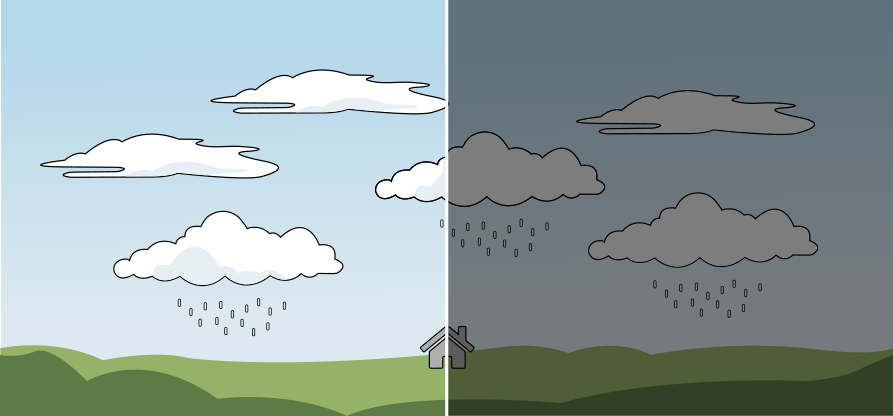
\includegraphics[width=0.8\textwidth]{rain proxy.png}};

        % tile label 1
        \draw (-0.7,4) -- (6.9,4);
        \draw (-0.7,3.95) -- (-0.7,4.05);
        \draw (6.9,3.95) -- (6.9,4.05);
        \node at (3.1,4.3) {no proxy};
        
        % tile label 2
        \draw (7,-4) -- (14.7,-4);
        \draw (7,-3.95) -- (7,-4.05);
        \draw (14.7,-3.95) -- (14.7,-4.05);
        \node at (10.85,-4.3) {proxy in effect};
        
    \end{tikzpicture}
    \captionof{figure}{Desired effect of the rain \gls{proxyplane}.}
    \label{img:techimpl:rainproxy}
\end{figure}

\noindent
The other \gls{proxyobject}, \color{darkercyan}$P_{sky}$\color{black}, makes sure the sun is surrounded by a bright circle of the same color, supporting the strength of the sunlight in the sky.
This effect is most prominent when the sun is setting or rising, giving the scene a more vibrant and natural look.

\begin{figure}[H]
    \centering
    \begin{tikzpicture}[scale=0.8]
        \tikzset{edge/.style = {-{Latex[length=3mm]},shorten >= -4pt}}
        \tikzset{shortedge/.style = {shorten <=-4pt,shorten >= -4pt}}
        \tikzset{icon/.style = {font=\Large}}
        \tikzset{mini/.style = {font=\footnotesize}}
        \tikzset{tiny/.style = {font=\tiny}}

        % cloud layer boxes
        \node[inner sep=0pt] at (7,0) 
            {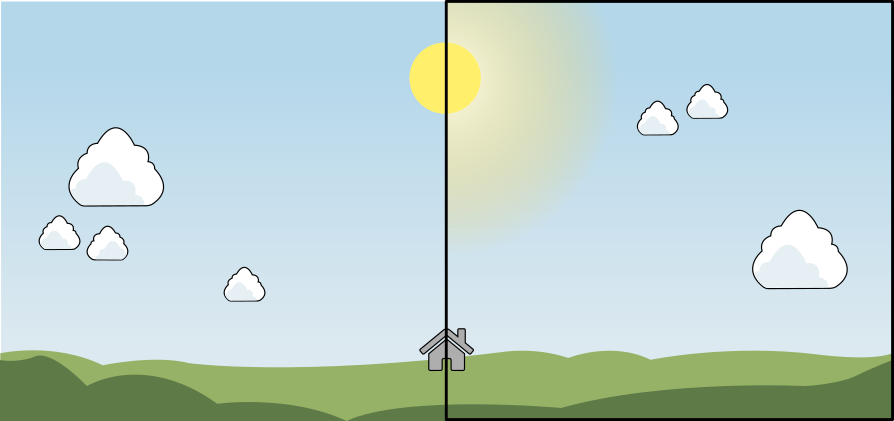
\includegraphics[width=0.8\textwidth]{sky proxy.png}};

        % tile label 1
        \draw (-0.7,4) -- (6.9,4);
        \draw (-0.7,3.95) -- (-0.7,4.05);
        \draw (6.9,3.95) -- (6.9,4.05);
        \node at (3.1,4.3) {no proxy};
        
        % tile label 2
        \draw (7,-4) -- (14.7,-4);
        \draw (7,-3.95) -- (7,-4.05);
        \draw (14.7,-3.95) -- (14.7,-4.05);
        \node at (10.85,-4.3) {proxy in effect};
        
    \end{tikzpicture}
    \captionof{figure}{Desired effect of the sky \gls{proxyplane}.}
    \label{img:techimpl:skyproxy}
\end{figure}

\noindent
This effect could also be implemented in the skybox, but with the skybox of the \gls{hdrp} being part of the \gls{pp}, it is easier to maintain a \gls{proxyobject} than to create a custom \gls{pp} effect.

\clearpage

\subsection{Render Process}
\label{section:techimpl:process}
Each component in the scene fulfills a specific role. The following graphic lists the tasks that each component has to do during the start of the simulation (OnStart), and during each \gls{updateloop} (OnUpdate).

\begin{figure}[H]
    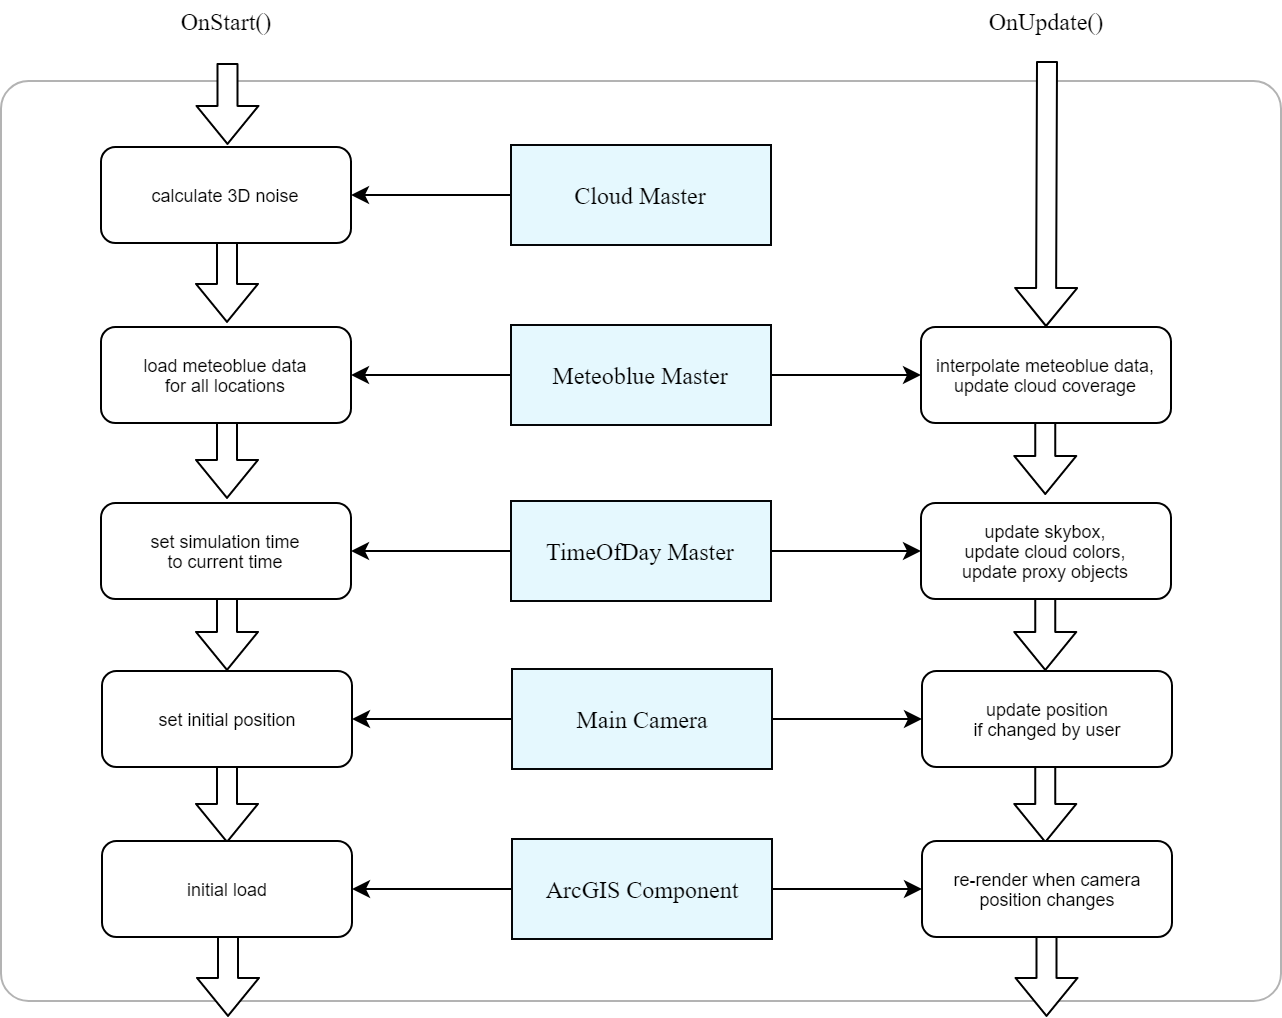
\includegraphics[width=\linewidth]{render process.png}
    \caption{Render process of the Unity project implementation.}
\end{figure}

\noindent
Since the 3D \gls{noise} texture, that is generated at the start by the "cloud master", is seamless, it does not have to be recalculated every frame.
After the \emph{meteoblue} data is loaded by the "meteoblue master", the setup is almost complete.
The default values for time of day and camera position are set while the \emph{ArcGIS} component starts itself and runs automatically.
\emptyline
During the update loop of the engine, the weather data is interpolated from hour to hour, depending on the current time.
This is necessary as the \emph{meteoblue} data is only available for every full hour.
This pseudo-code snippet shows how an average value for the weather data would be determined based on the time.

\begin{lstlisting}[language=HLSL, caption=Pseudo-code for linear interpolation of weather data., label=lst:psuedo:weather:lerp]
simulationTime = "18:45" // current simulation time (24h-clock)
time1 = floor(simulationTime) // "18:00"
time2 = ceil(simulationTime) // "19:00"
x = lerp(time1, time2, simulationTime) // 0.75

weatherData = lerp(weatherDataFor(time1), weatherDataFor(time2), x)
\end{lstlisting}

\clearpage

\subsection{Noise Generation}
\label{section:techimpl:noise}
As extensively described in \sectionref{section:noise}, the \gls{noise} texture is generated by a \gls{computeshader}.
The resulting 3D texture is seamless and is solely based on the Voronoi \gls{noisegeneration} algorithm, invoked with different scales and octaves.
In the output texture, each \gls{texel} holds four different \gls{noise} values, one for each color channel.
\\
The compute shader is dispatched only once, at the start of the simulation.
This saves on a great deal of performance, as the \gls{noise} does not need to be recalculated each frame.

\subsection{Rendering Techniques}
As mentioned in \sectionref{section:noise:previous}, algorithms that have been documented in the previous project will not be described again.
The current solution uses techniques like \gls{raymarching}, \gls{lightmarching} and \gls{sunlightforwarding} in a very similar fashion.

\subsection{Shadow Casting}
\label{section:techimpl:shadow}
The \gls{volumetric} cloud \gls{shader}s do not contain a \gls{shadowpass}, which means that the cloud objects do not cast shadows themselves.
This is associated with the \emph{ArcGIS}  component.
\\
The \emph{ArcGIS} plugin generates geometry with an extremely high scale, where one \gls{inengine} unit corresponds to one meter in real life.
The resulting geometry is huge compared to the rest of the scene. This is a problem, because the map's dimension exceed the capabilities and size of Unity's shadow texture.
Unfortunately the geometry cannot be reduced in size so easily, because when reducing the scale of the generated map, the textures lose a good amount of detail.
\\
However, the problem was solved with an alternative approach to casting shadows.

\begin{figure}[H]
    \centering
        \begin{minipage}{0.47\linewidth}
            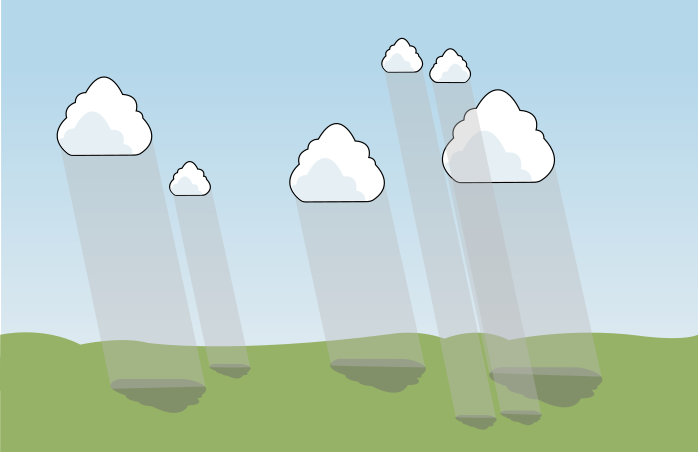
\includegraphics[width=\linewidth]{shadowcasting1.png}
            \captionof{figure}{Shadow casting: Normally, objects would cast their own shadow in a dedicated \gls{shadowpass}.}
            \label{img:shadow:casting1}
        \end{minipage}
    \hfill
        \begin{minipage}{0.47\linewidth}
            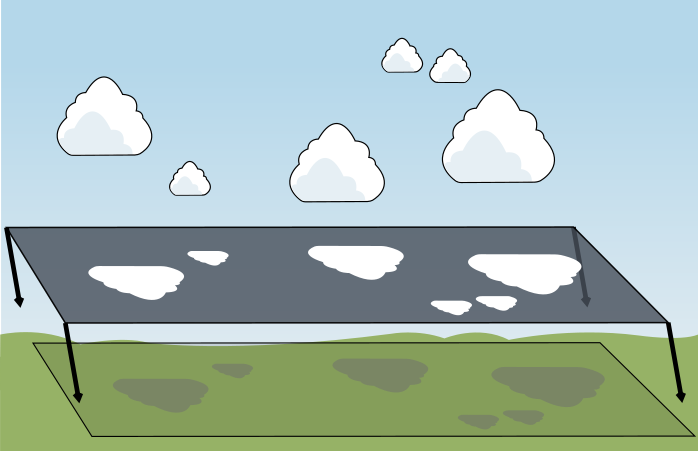
\includegraphics[width=\linewidth]{shadowcasting2.png}
            \captionof{figure}{Shadow casting substitution: The 3D \gls{noise} texture is sampled again in the ground shader and added as shadow.}
            \label{img:shadow:casting2}
        \end{minipage}
\end{figure}

\noindent
What \autoref{img:shadow:casting2} shows is not a plane that casts the shadow, but instead an illustration of how the data is used from the same \gls{noise} texture that was used for the clouds.
Thus, the shader for the ground tile, which is provided by the \emph{ArcGIS} plugin, was modified to read the 3D \gls{noise} texture.
With that information, the ground shader knows where the clouds will be in the sky and adds a darkened, transparent layer over the existing ground color.
\emptyline
This method works well for the current solution, but would there be other objects than clouds, they would not cast shadows for the same reasons.

\clearpage

\subsection{Results}
\label{section:techimpl:results}
The final implementation yields great results, visualizing the \emph{meteoblue} weather reports in a variety of different settings, at all times of day.

\subsection{Cloud Layers}
As displayed in \autoref{img:result:anatomy}, each cloud layer renders an approximation of the clouds it represents.
In the low-level layer, there are small puffy \gls{cloudlet}s. In the alto-layer, there are dense fields of clouds and lastly, the distant cloud layer shows high-towering heaps of cumulonimbus approximations.

\begin{figure}[H]
    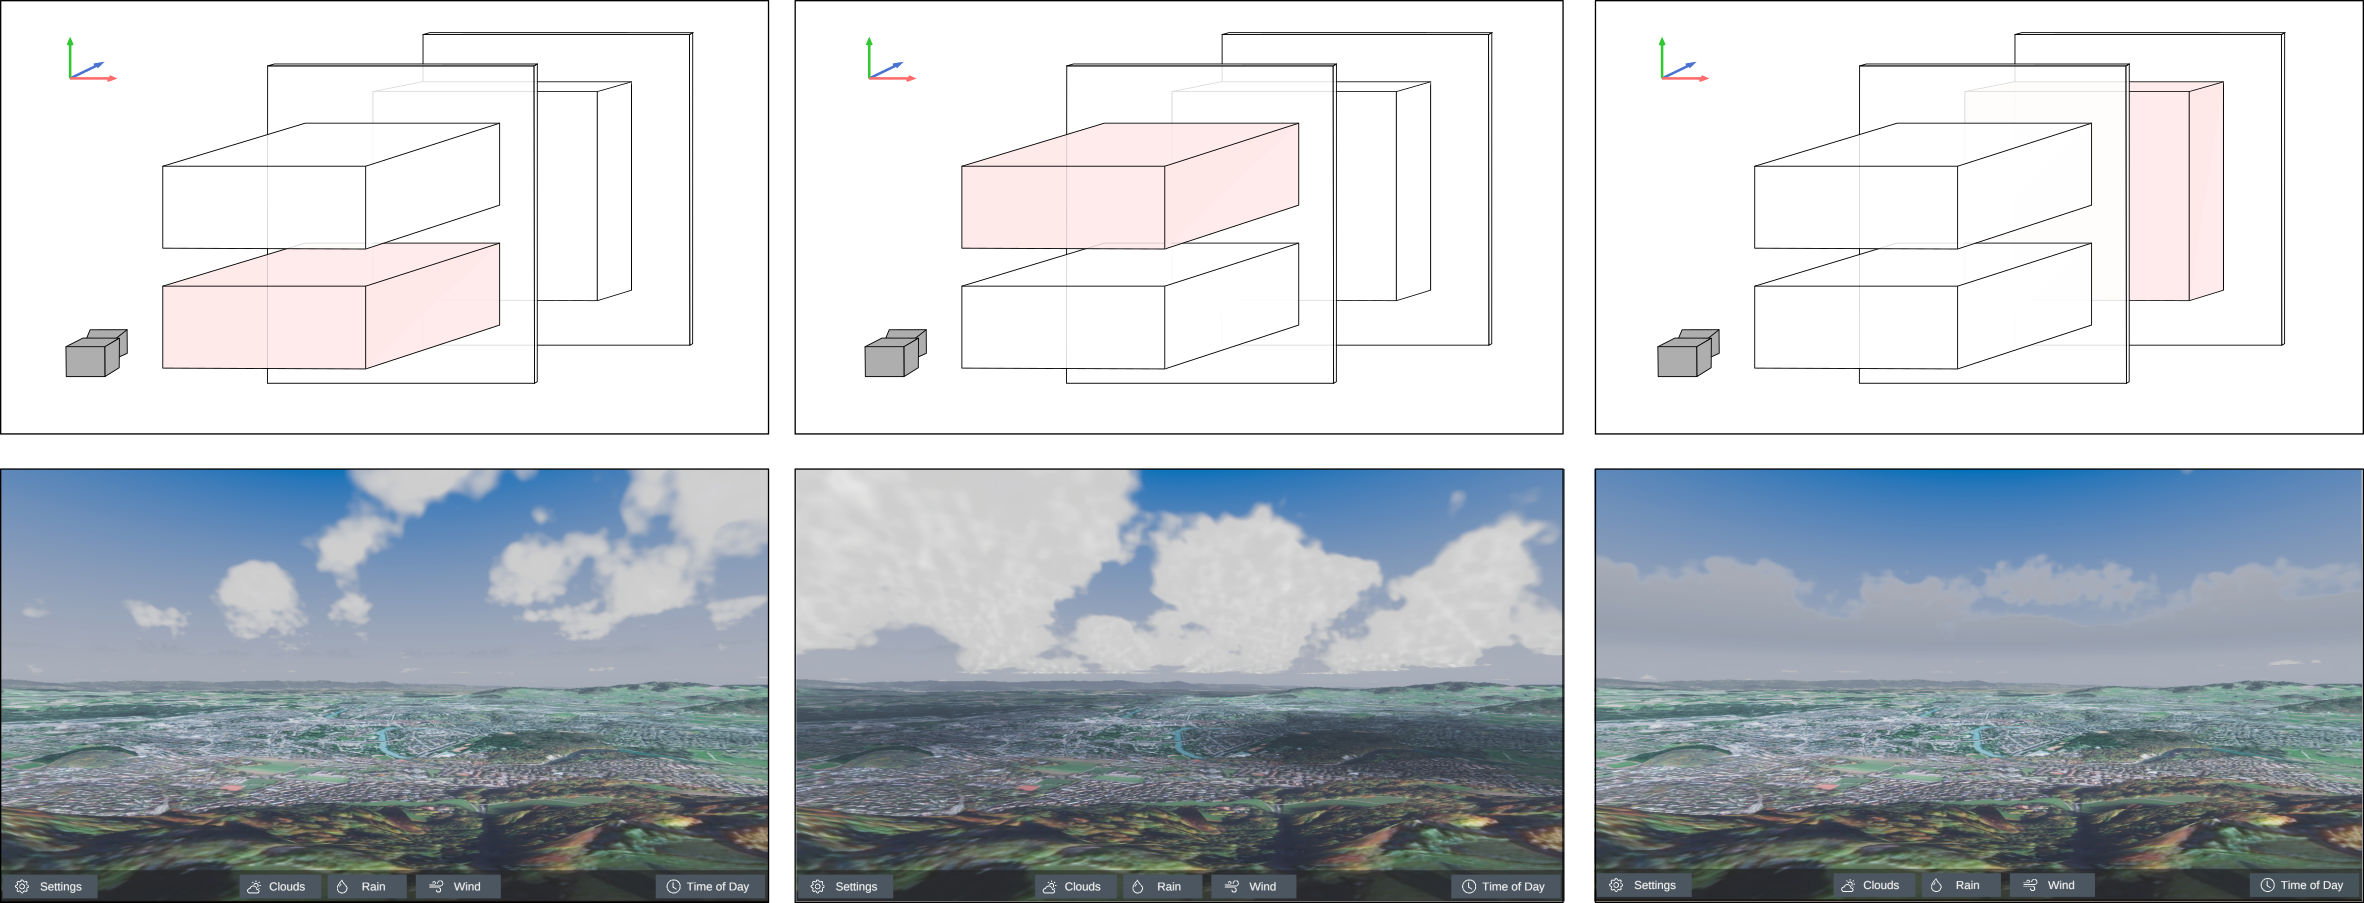
\includegraphics[width=\linewidth]{anatomy_result.png}
    \caption{Side-by-side comparison of the cloud layers and their visual outputs.}
    \label{img:result:anatomy}
\end{figure}

\noindent
Combined, the final output shows a diverse scene for the weather conditions extracted from the \emph{meteoblue} data.

\begin{figure}[H]
    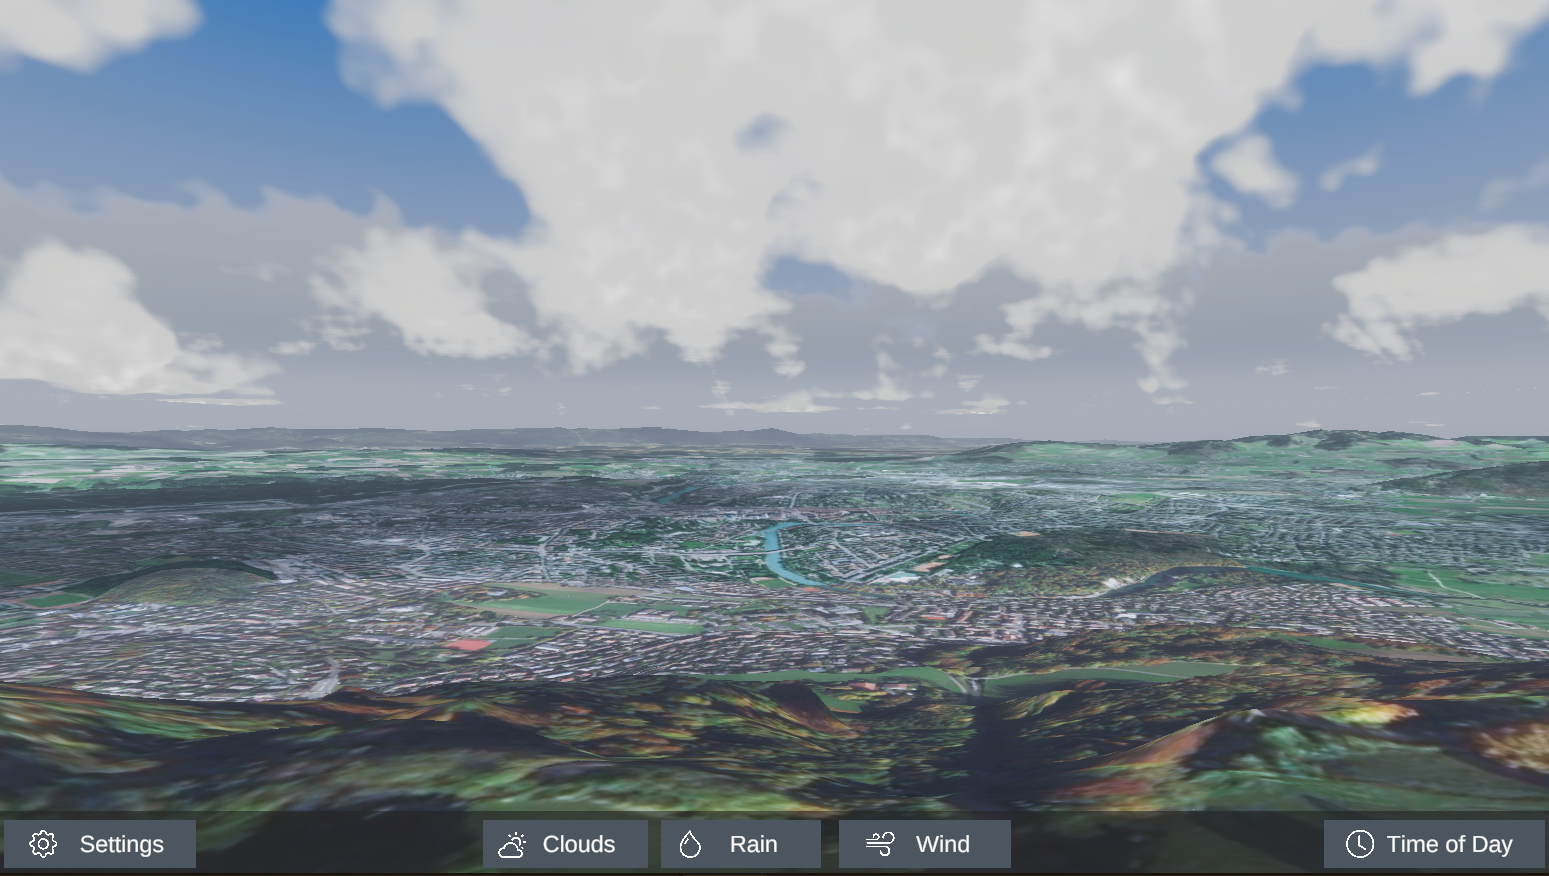
\includegraphics[width=\linewidth]{anatomy/all.png}
    \caption{Final render output of the weather rendering system.}
    \label{img:result:final1}
\end{figure}

\clearpage

\subsubsection{Times Of Day}
The current solution is able to render the weather for all times of day. The following figures demonstrate the capabilities of the weather rendering system.

\begin{figure}[H]
    \centering
        \begin{minipage}{0.47\linewidth}
            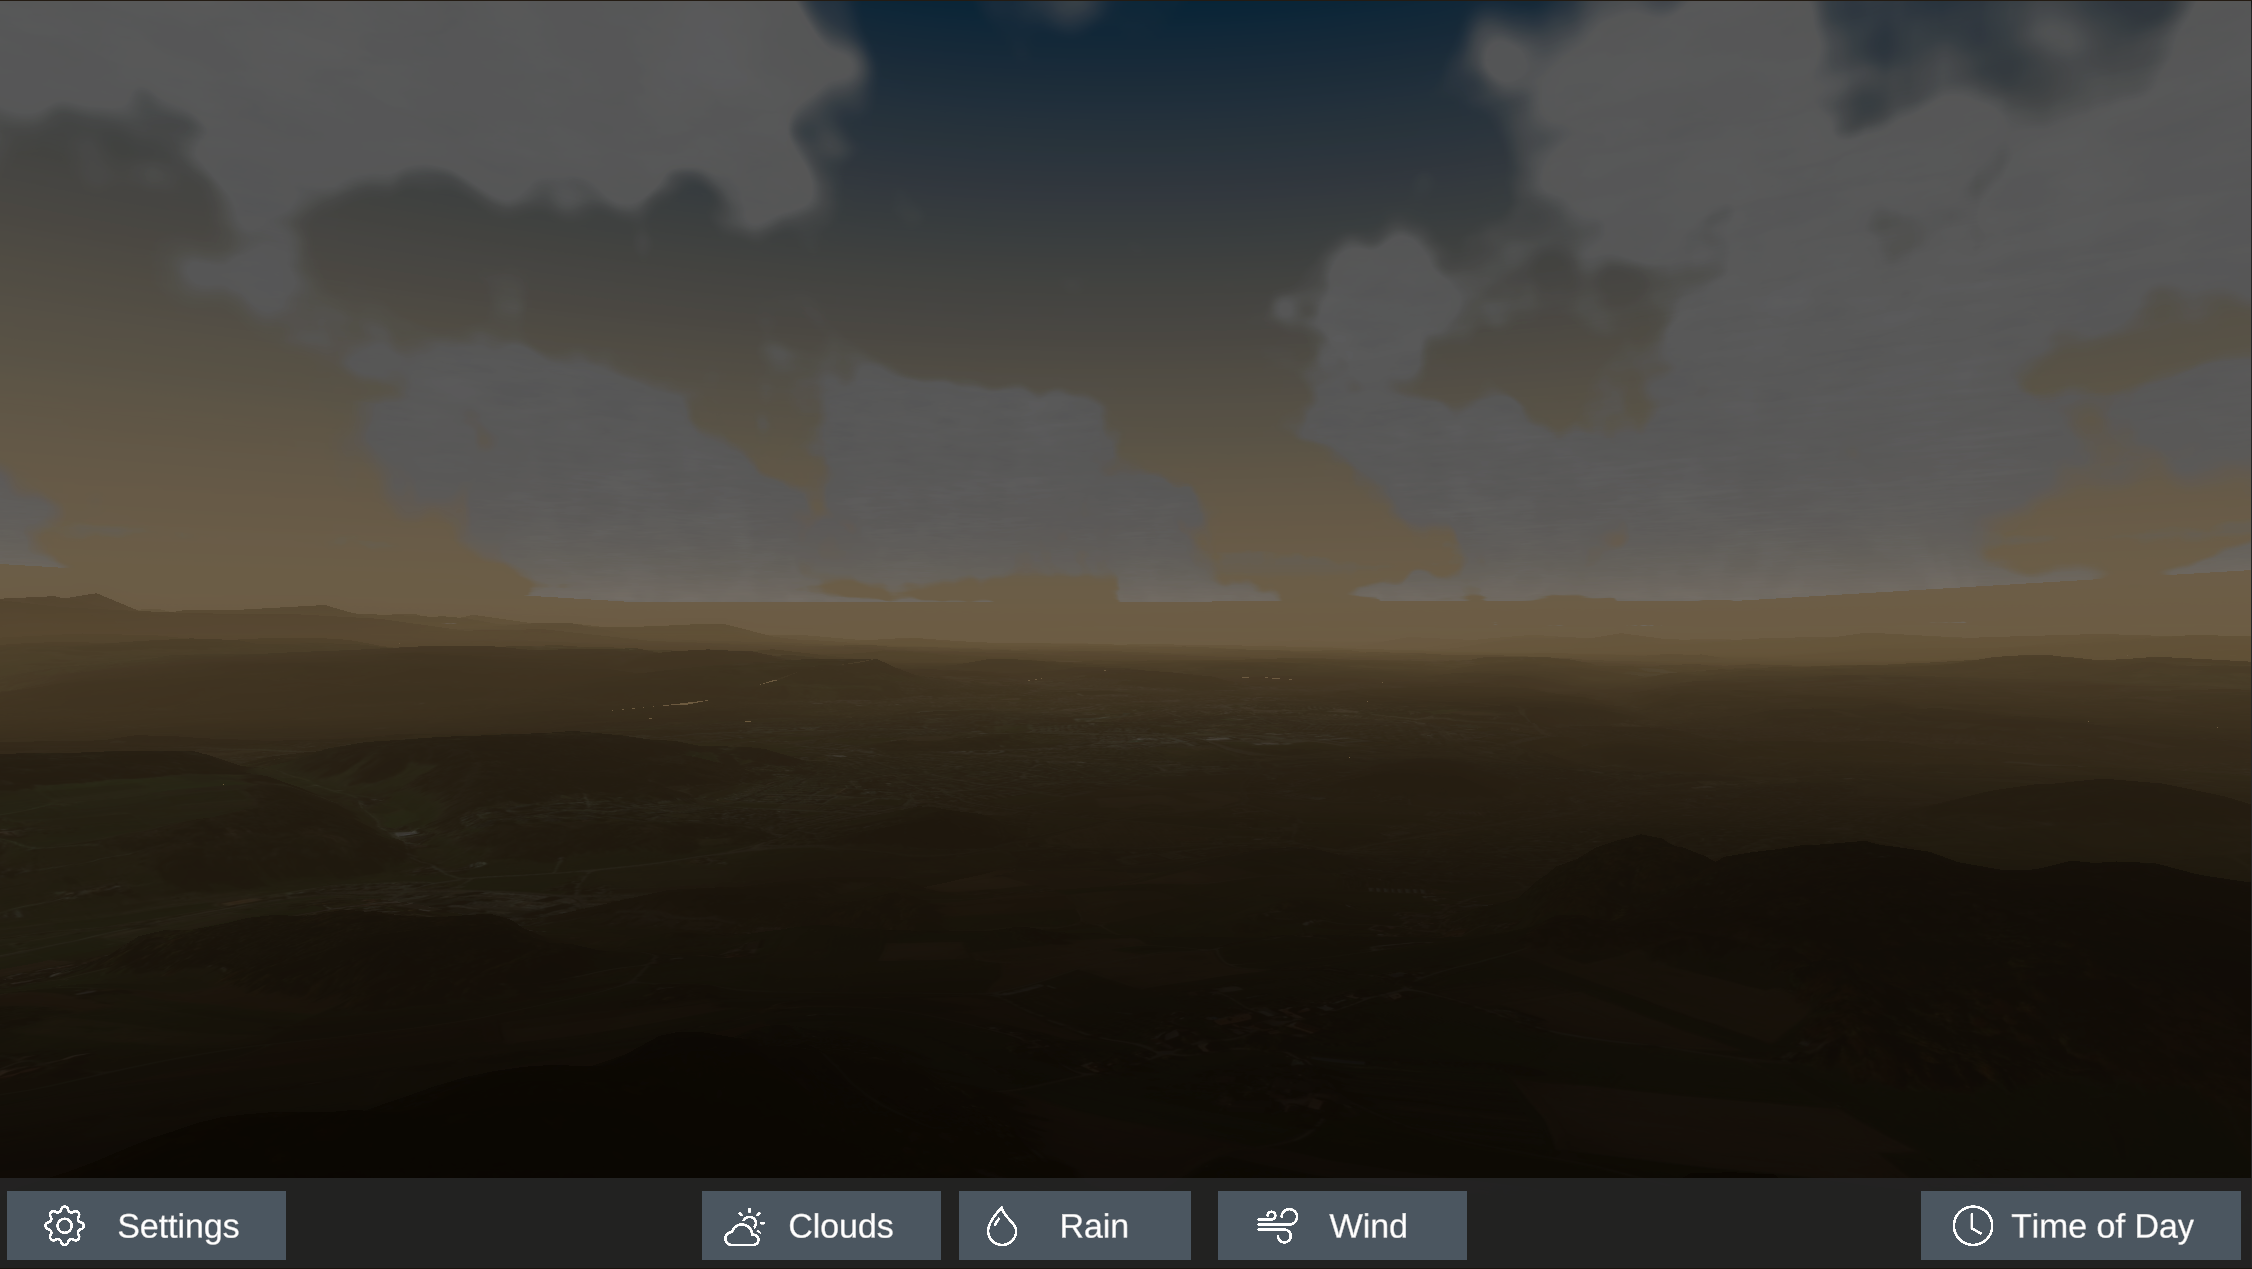
\includegraphics[width=\linewidth]{results/wheel1.png}
            \captionof{figure}{Final render output for a partly cloudy morning before sunrise.}
            \label{img:result:1}
        \end{minipage}
    \hfill
        \begin{minipage}{0.47\linewidth}
            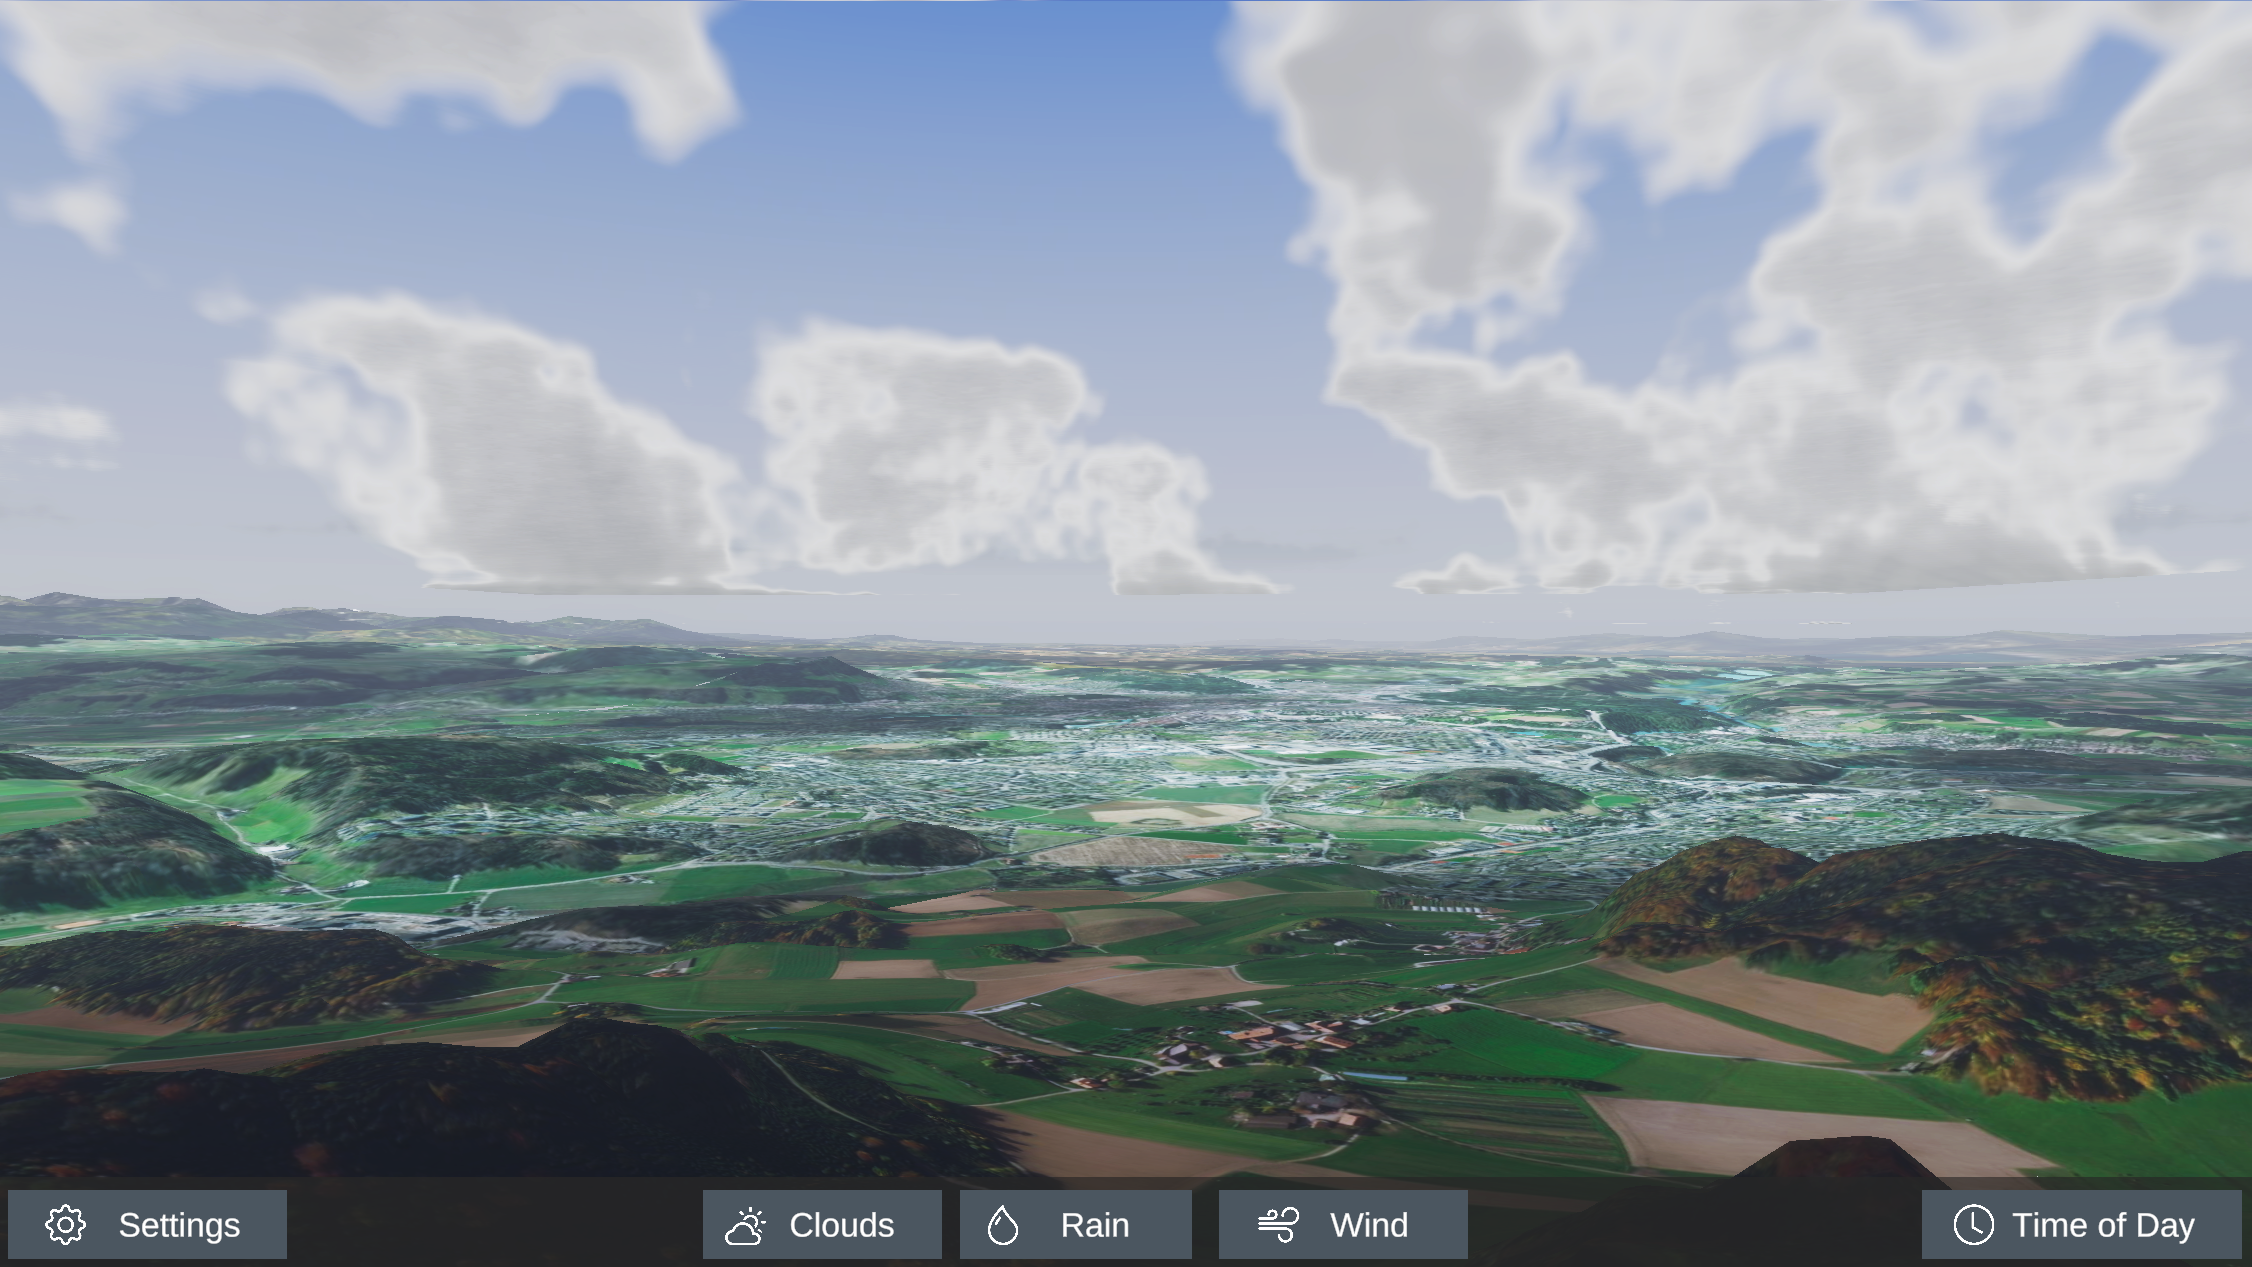
\includegraphics[width=\linewidth]{results/wheel2.png}
            \captionof{figure}{Final render output for a early afternoon.}
            \label{img:result:2}
        \end{minipage}
\end{figure}


\begin{figure}[H]
    \centering
        \begin{minipage}{0.47\linewidth}
            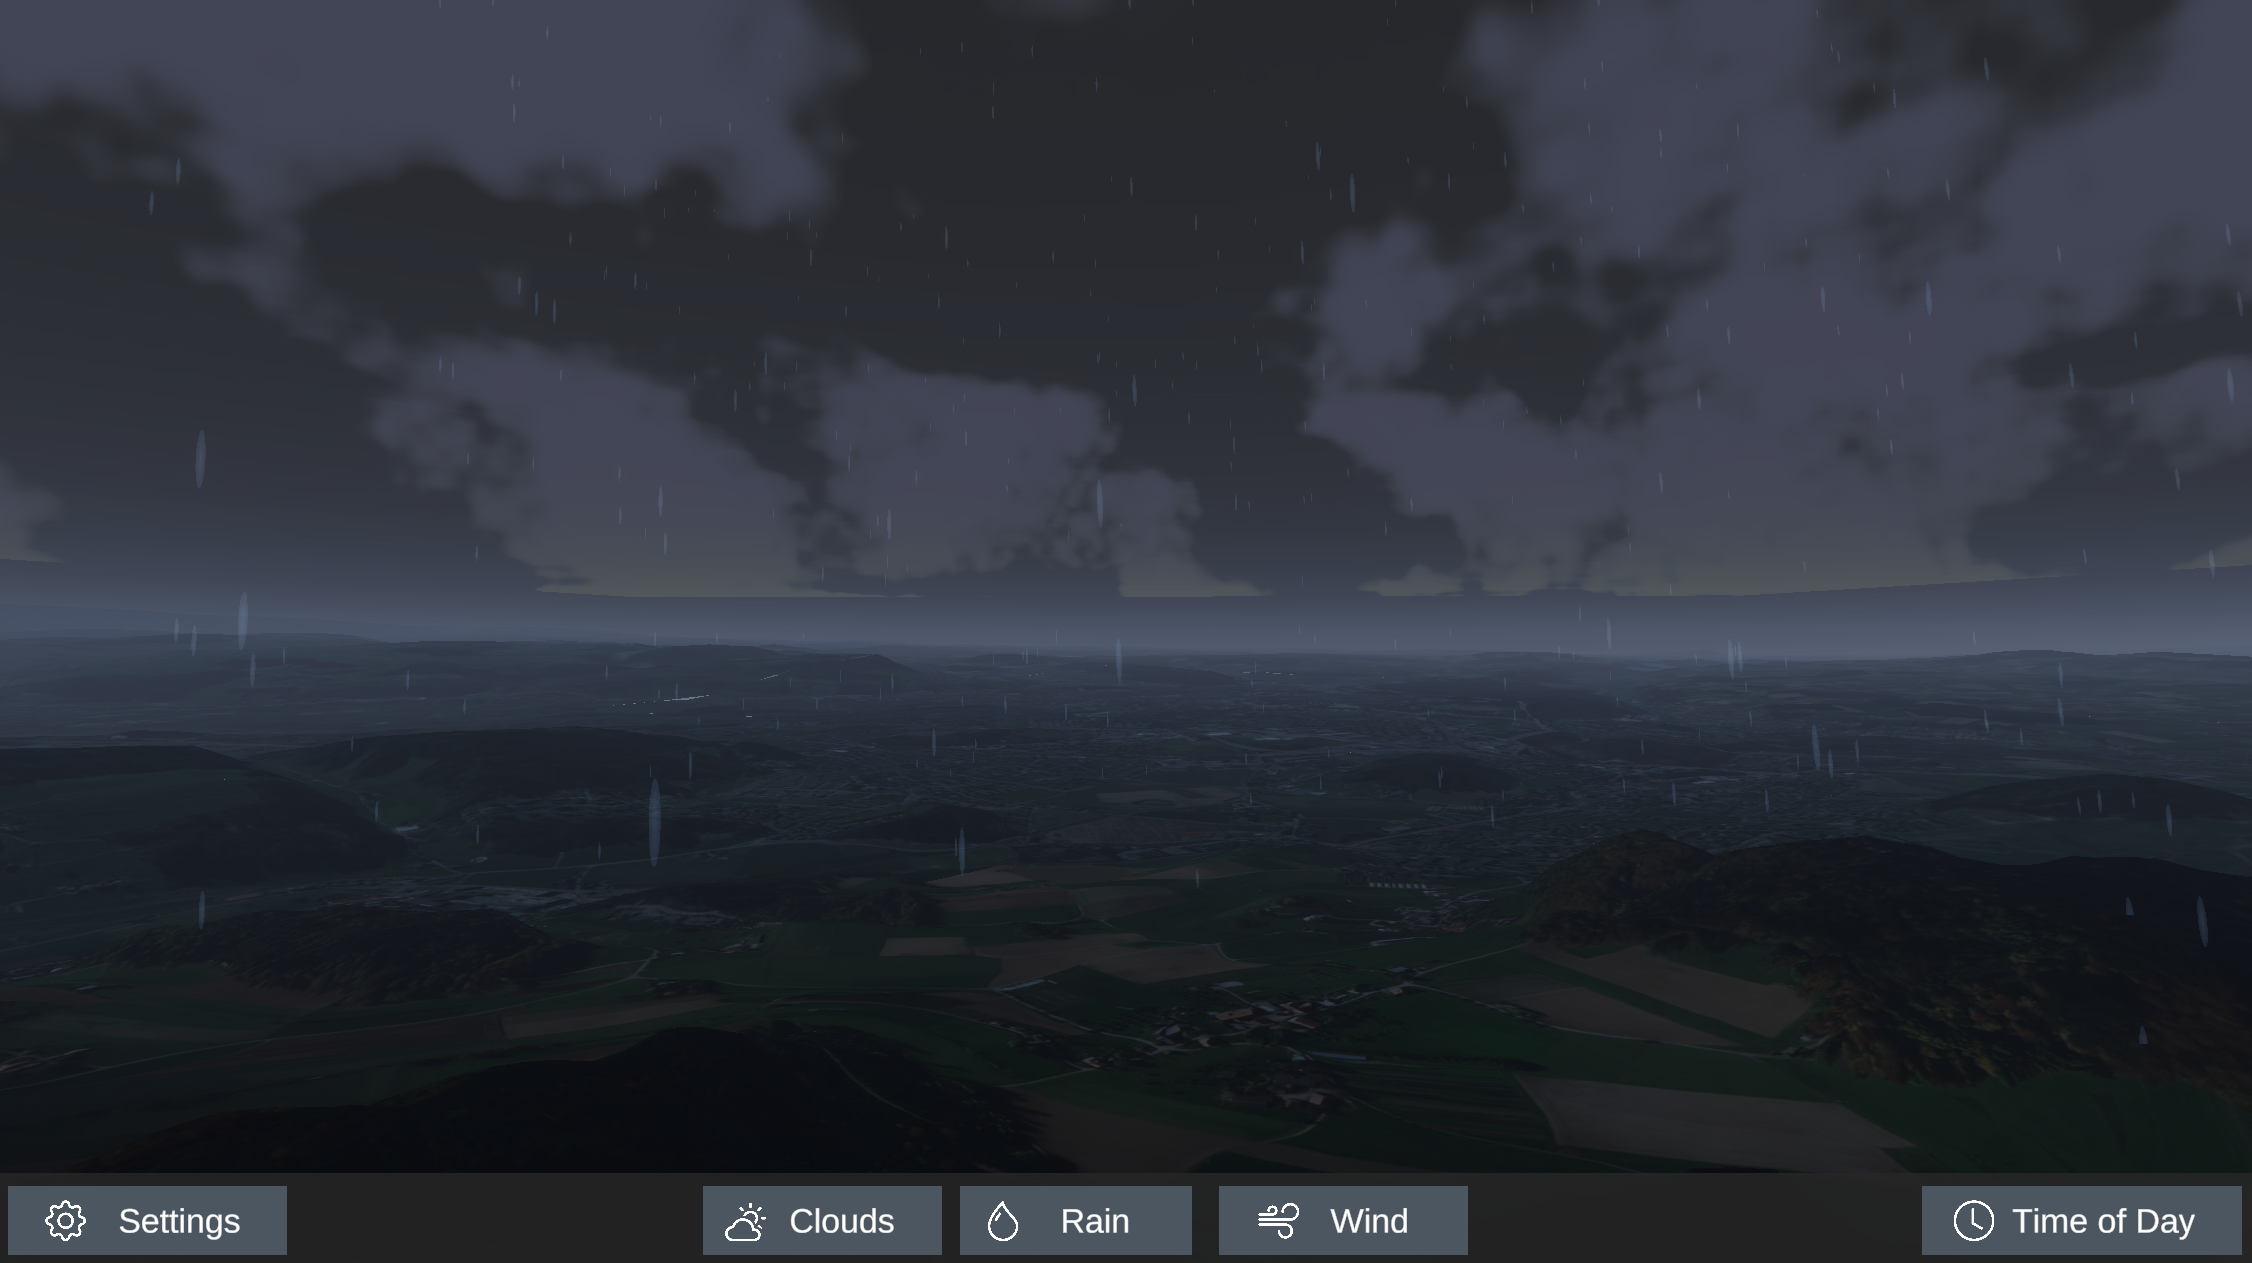
\includegraphics[width=\linewidth]{results/wheel3.png}
            \captionof{figure}{Final render output for a rainy evening.}
            \label{img:result:3}
        \end{minipage}
    \hfill
        \begin{minipage}{0.47\linewidth}
            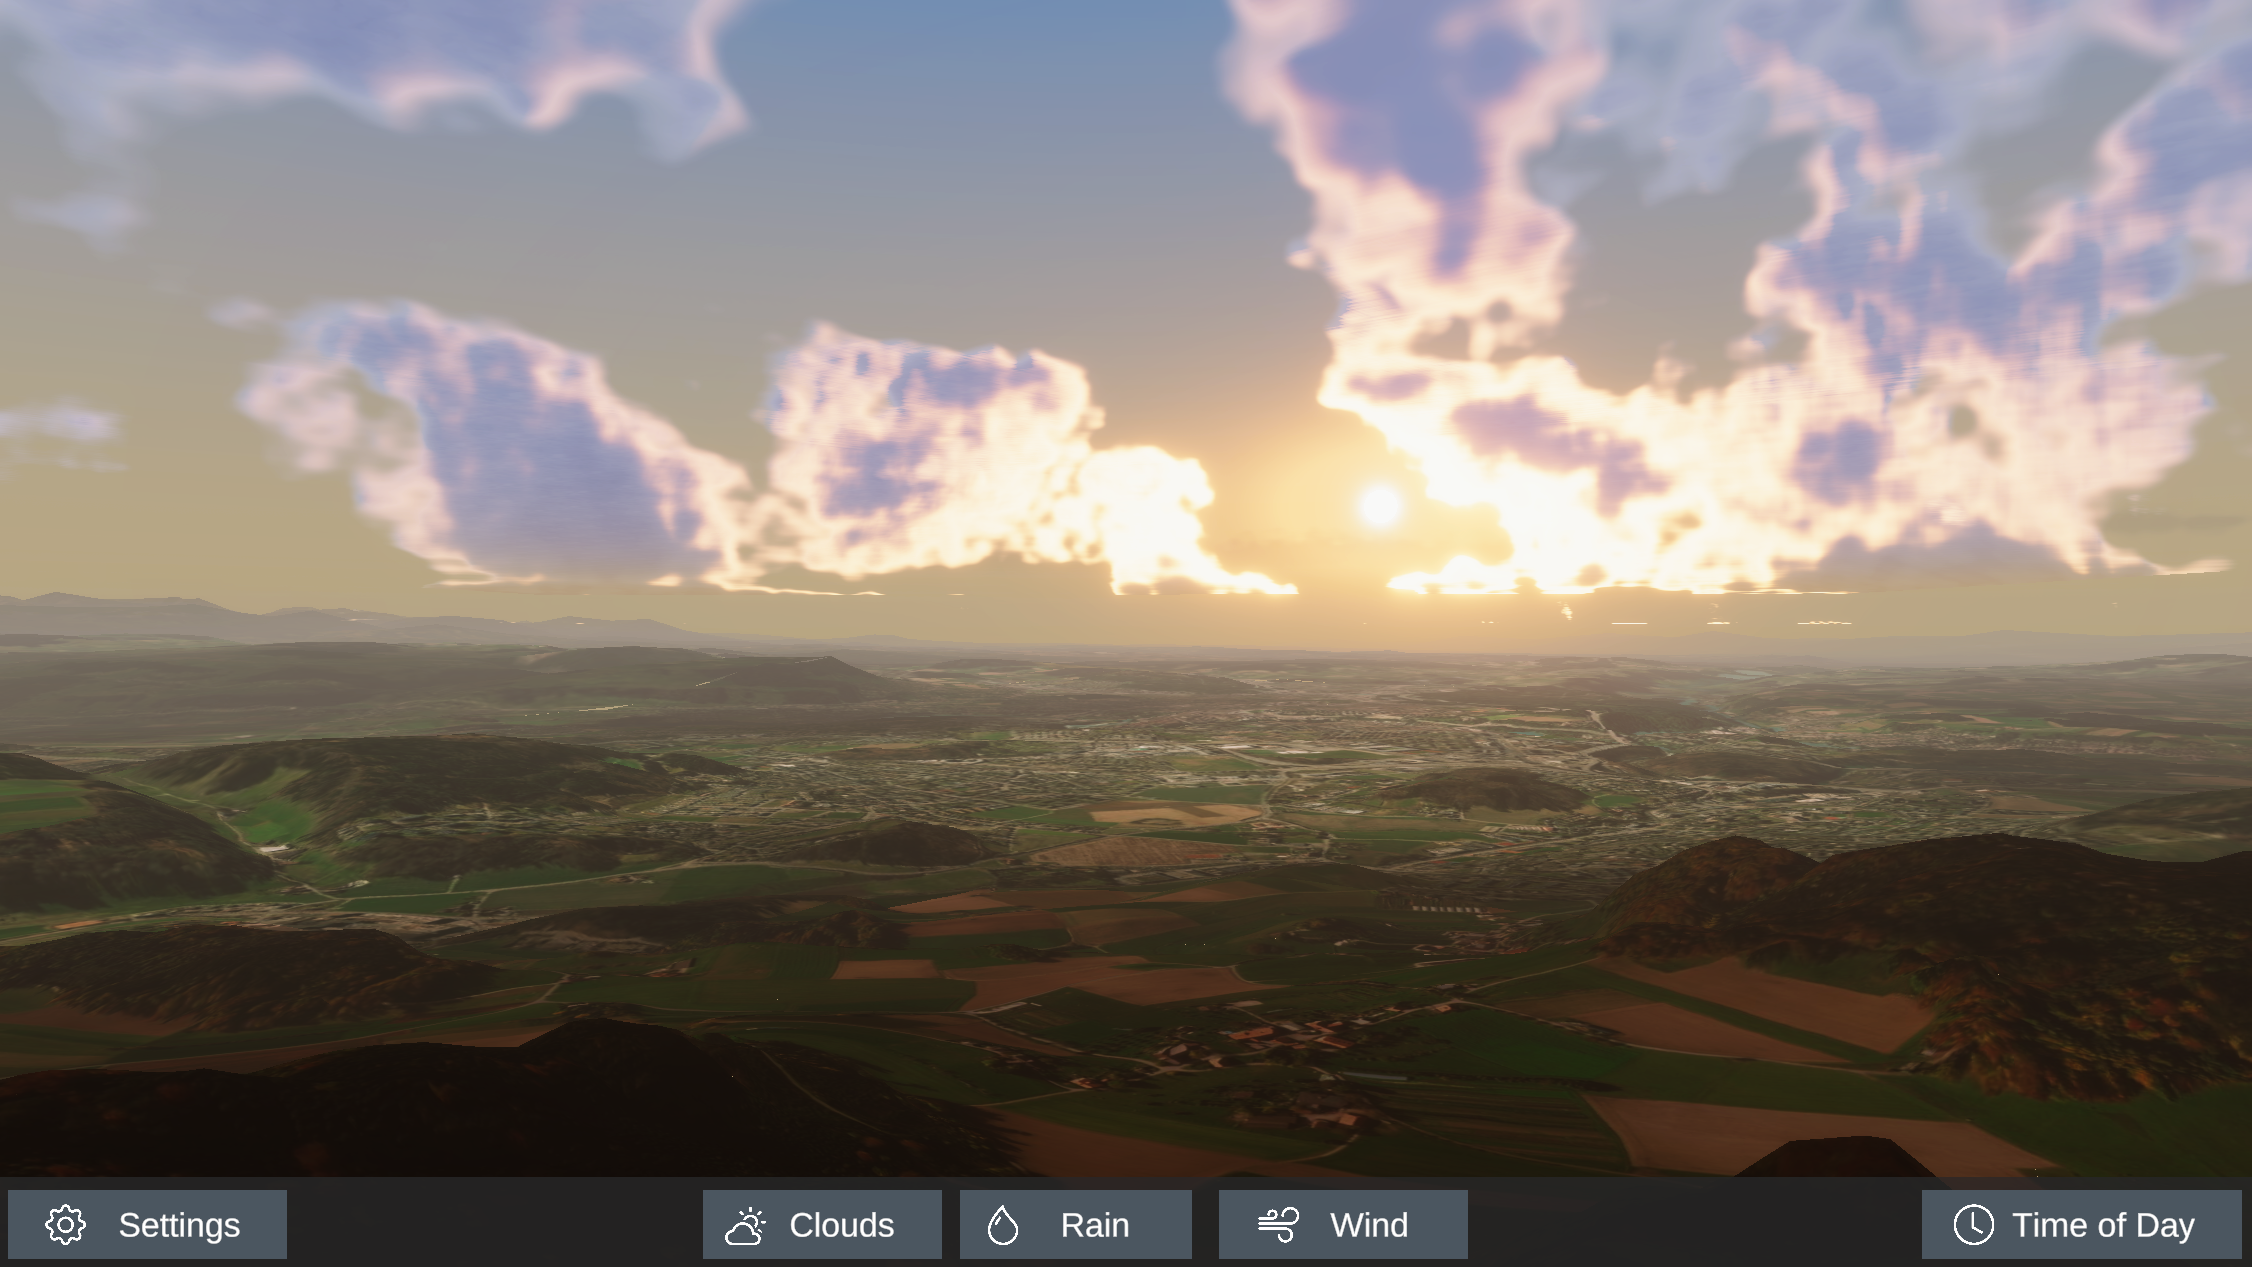
\includegraphics[width=\linewidth]{results/wheel4.png}
            \captionof{figure}{Final render output for a golden sunset.}
            \label{img:result:4}
        \end{minipage}
\end{figure}


\begin{figure}[H]
    \centering
        \begin{minipage}{0.47\linewidth}
            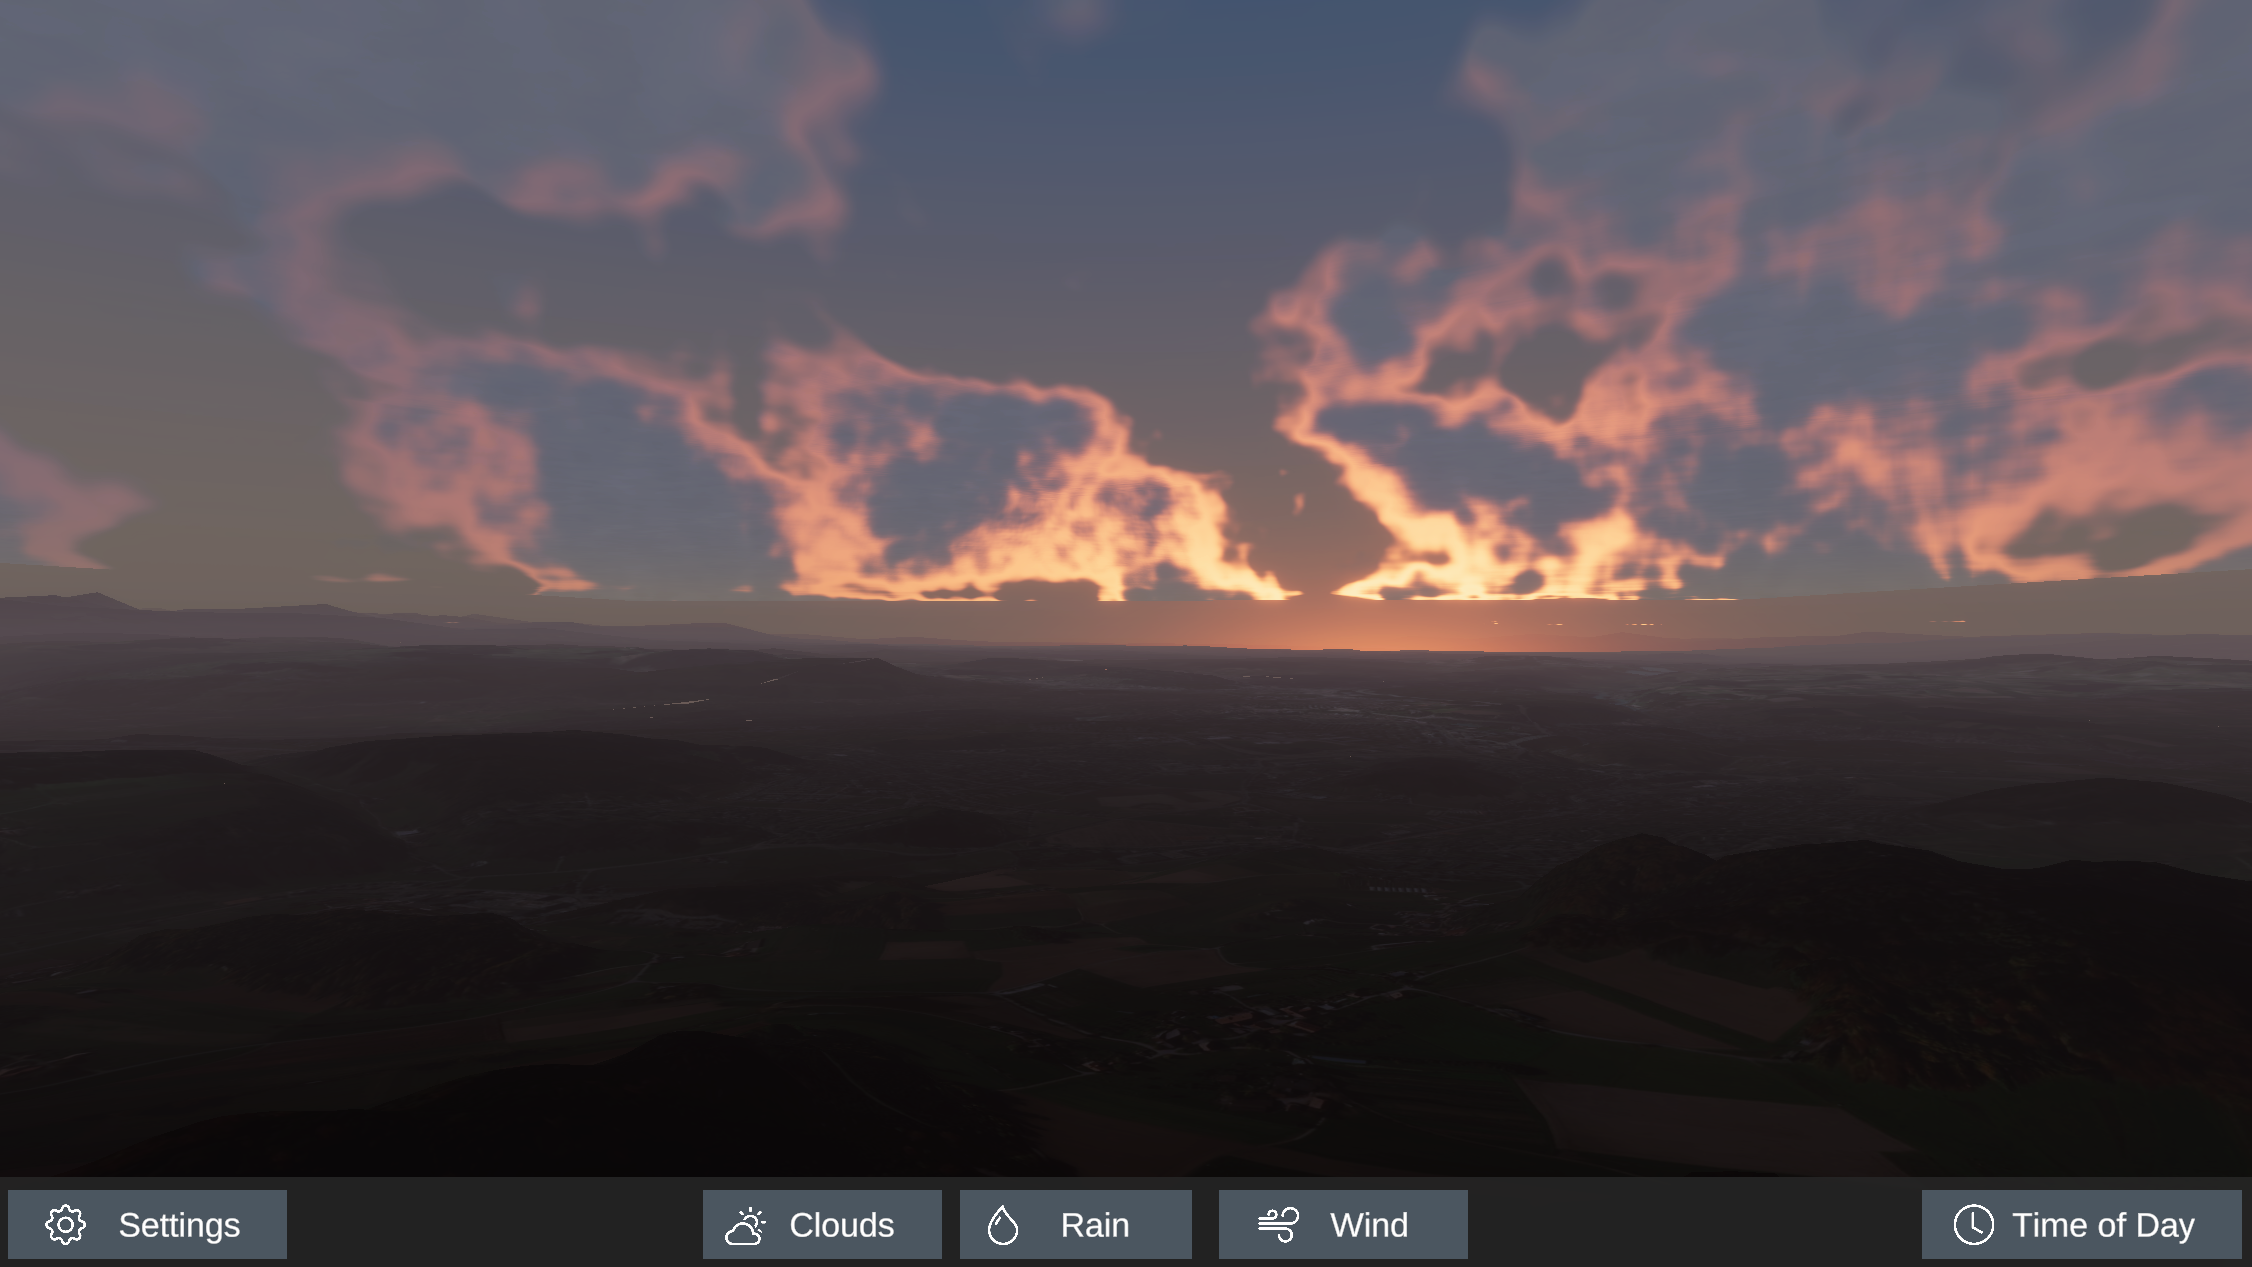
\includegraphics[width=\linewidth]{results/wheel5.png}
            \captionof{figure}{Final render output for a evening right after sunset.}
            \label{img:result:5}
        \end{minipage}
    \hfill
        \begin{minipage}{0.47\linewidth}
            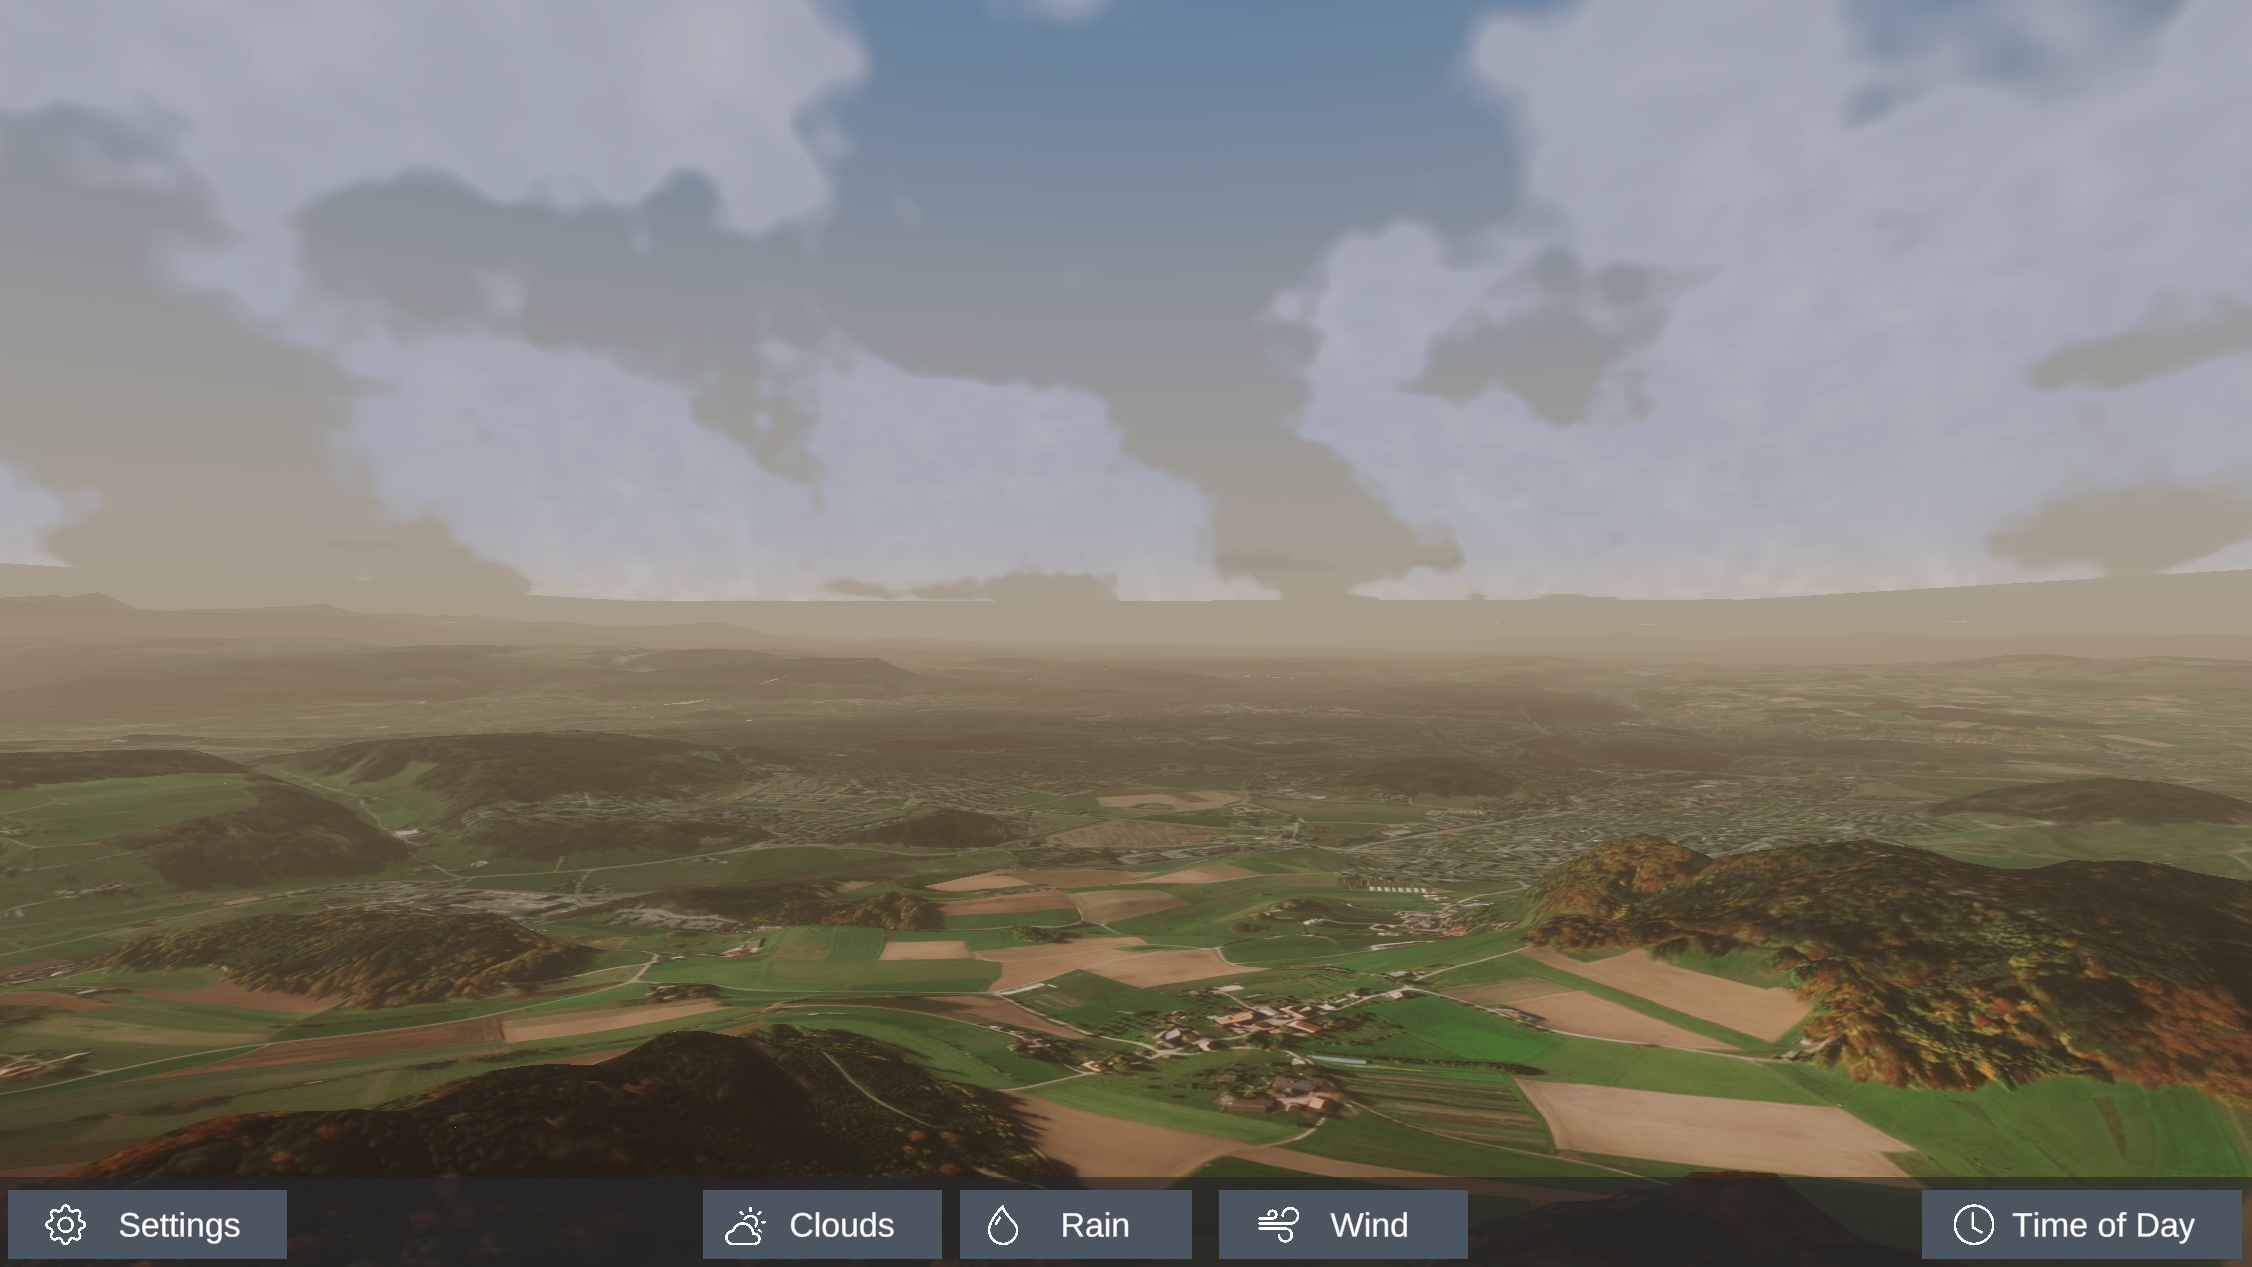
\includegraphics[width=\linewidth]{results/wheel6.png}
            \captionof{figure}{Final render output for a cloudy morning.}
            \label{img:result:6}
        \end{minipage}
\end{figure}

\noindent
the colors of the clouds are influenced by the skybox and the sun's light. They also adapt to the amount of \gls{precipitation} as well as the fog color.
The clouds have an outer and inner primary color, both enriched with details from the \gls{noise} texture.
The outer edge of the clouds reacts the most to the sun's position and intensity, especially improving the scene at sunrise and sunset.

\clearpage

\subsubsection{Proxy Objects}
The \gls{proxyobject}s were used instead of complex, custom \gls{pp} effects. Their effects are key to the credibility of realism of the rendered scenes.
As the following graphics show, the \gls{proxyplane}s add a vital visual upgrade to the scenery.
\begin{figure}[H]
    \centering
    \begin{tikzpicture}[scale=0.8]
        \tikzset{edge/.style = {-{Latex[length=3mm]},shorten >= -4pt}}
        \tikzset{shortedge/.style = {shorten <=-4pt,shorten >= -4pt}}
        \tikzset{icon/.style = {font=\Large}}
        \tikzset{mini/.style = {font=\footnotesize}}
        \tikzset{tiny/.style = {font=\tiny}}

        % cloud layer boxes
        \node[inner sep=0pt] at (7,0) 
            {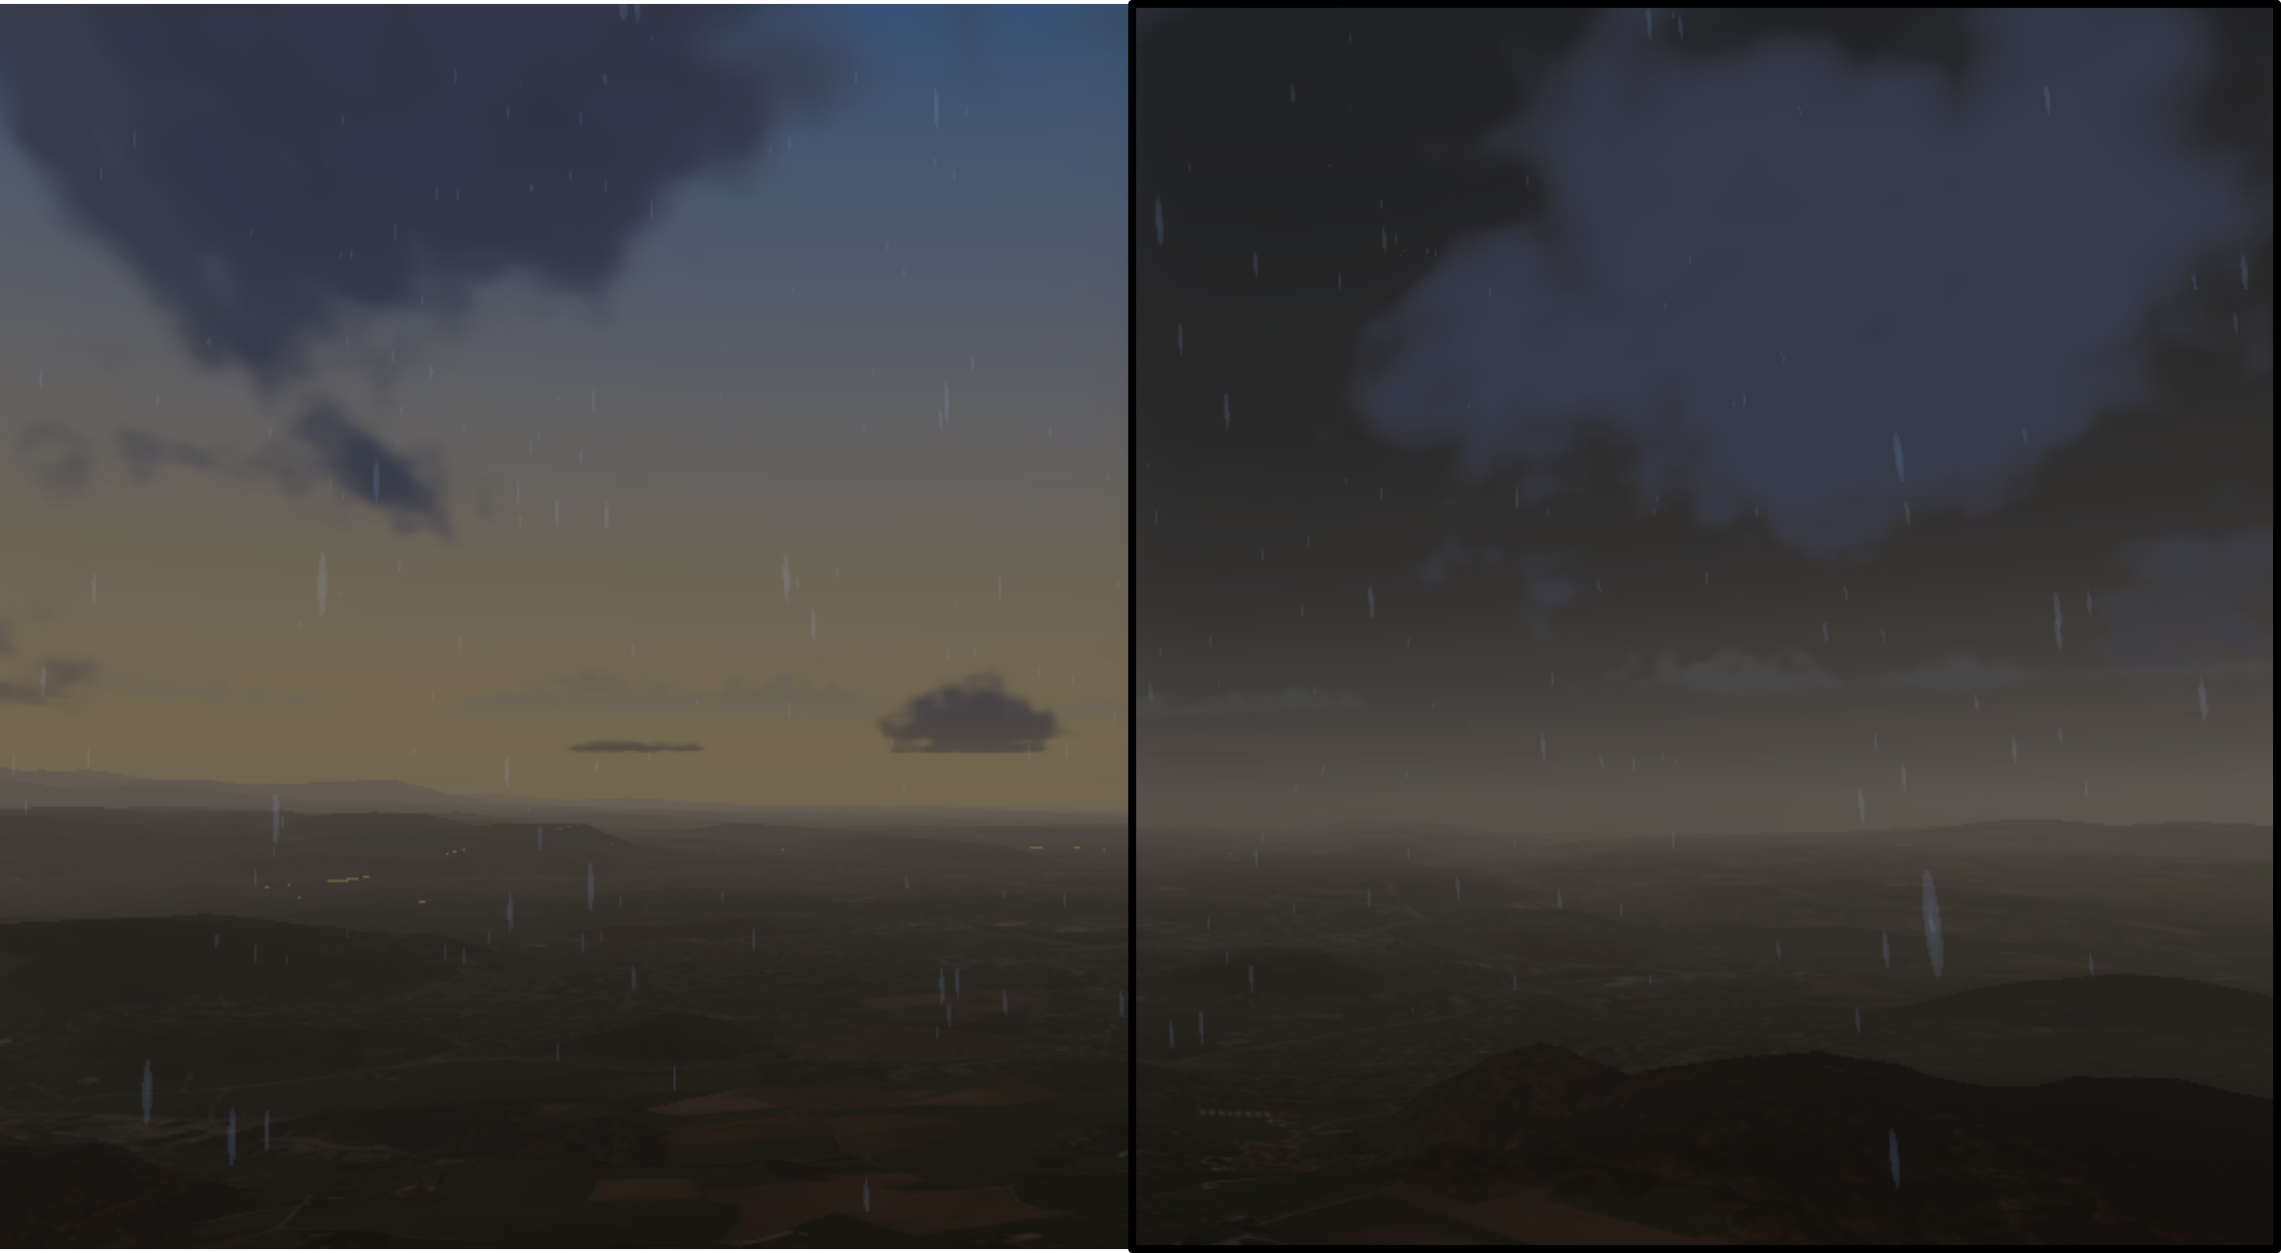
\includegraphics[width=0.8\textwidth]{results/rainproxy.png}};

        % tile label 1
        \draw (-0.7,4.4) -- (6.9,4.4);
        \draw (-0.7,4.35) -- (-0.7,4.45);
        \draw (6.9,4.35) -- (6.9,4.45);
        \node at (3.1,4.7) {no proxy};
        
        % tile label 2
        \draw (7,-4.4) -- (14.7,-4.4);
        \draw (7,-4.35) -- (7,-4.45);
        \draw (14.7,-4.35) -- (14.7,-4.45);
        \node at (10.85,-4.7) {proxy in effect};
        
    \end{tikzpicture}
    \captionof{figure}{Visual comparison of a rendered scene with and without the rain \gls{proxyplane}.}
    \label{img:results:rainproxy}
\end{figure}

\begin{figure}[H]
    \centering
    \begin{tikzpicture}[scale=0.8]
        \tikzset{edge/.style = {-{Latex[length=3mm]},shorten >= -4pt}}
        \tikzset{shortedge/.style = {shorten <=-4pt,shorten >= -4pt}}
        \tikzset{icon/.style = {font=\Large}}
        \tikzset{mini/.style = {font=\footnotesize}}
        \tikzset{tiny/.style = {font=\tiny}}

        % cloud layer boxes
        \node[inner sep=0pt] at (7,0) 
            {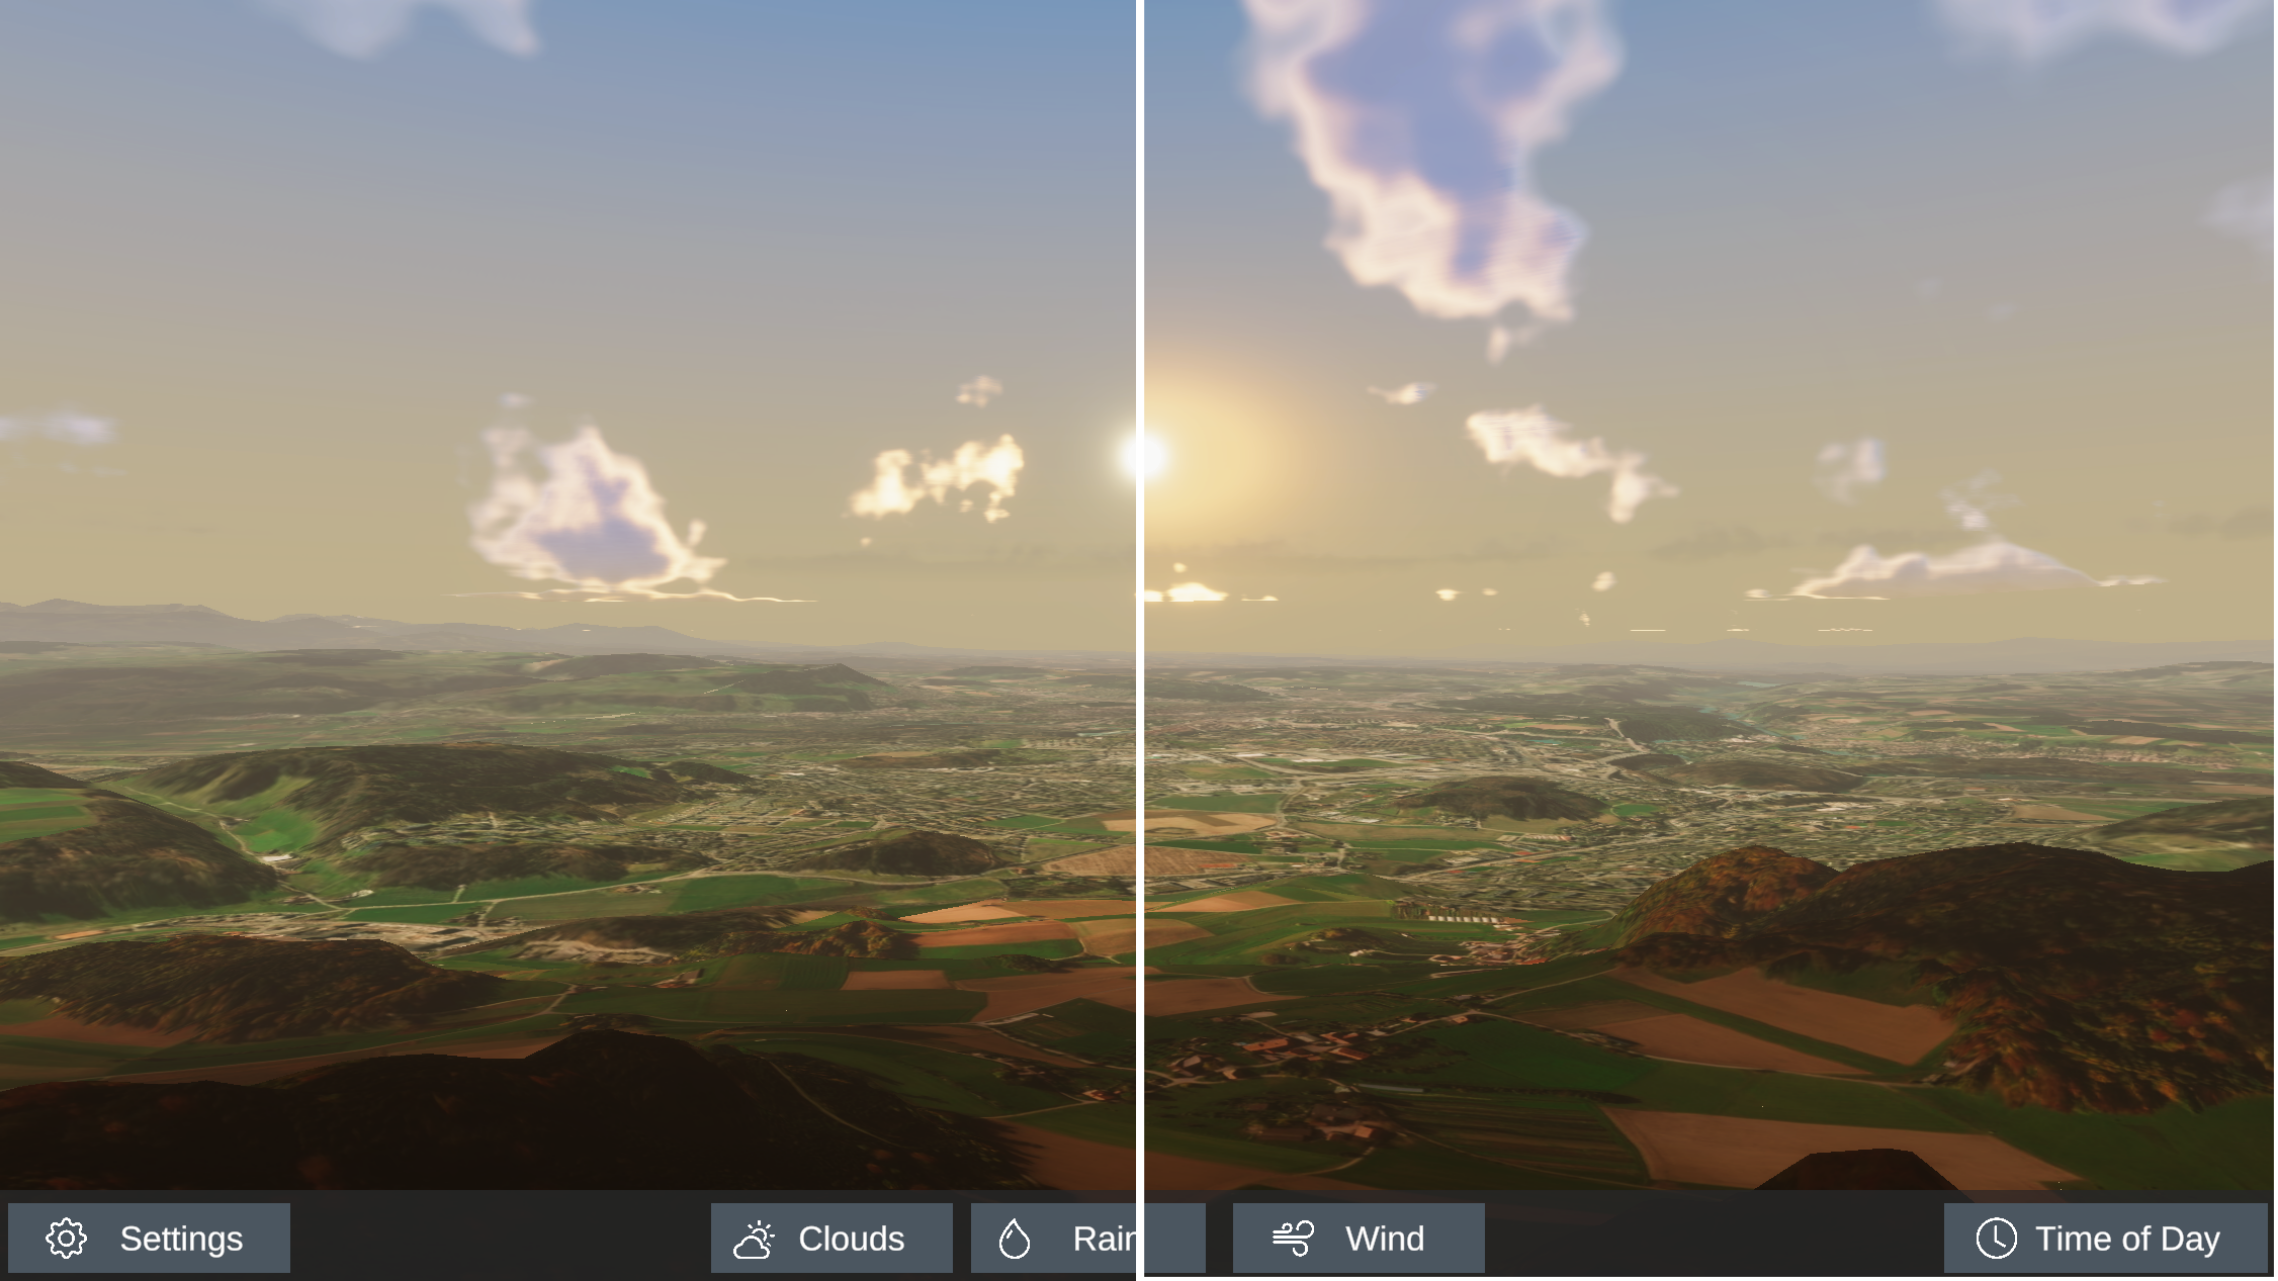
\includegraphics[width=0.8\textwidth]{results/skyproxy.png}};

        % tile label 1
        \draw (-0.7,4.4) -- (6.9,4.4);
        \draw (-0.7,4.35) -- (-0.7,4.45);
        \draw (6.9,4.35) -- (6.9,4.45);
        \node at (3.1,4.7) {no proxy};
        
        % tile label 2
        \draw (7,-4.4) -- (14.7,-4.4);
        \draw (7,-4.35) -- (7,-4.45);
        \draw (14.7,-4.35) -- (14.7,-4.45);
        \node at (10.85,-4.7) {proxy in effect};
        
    \end{tikzpicture}
    \captionof{figure}{Visual comparison of a rendered scene with and without the sky \gls{proxyplane}.}
    \label{img:results:skyproxy}
\end{figure}

\clearpage

\subsubsection{Shadow Mapping}
As described in \sectionref{section:techimpl:shadow}, the cloud objects do not cast shadows.
Instead, the terrain \gls{shader} was modified to read the 3D \gls{noise} texture and calculate the shadow itself .

\begin{figure}[H]
    \centering
    \begin{tikzpicture}[scale=0.8]
        \tikzset{edge/.style = {-{Latex[length=3mm]},shorten >= -4pt}}
        \tikzset{shortedge/.style = {shorten <=-4pt,shorten >= -4pt}}
        \tikzset{icon/.style = {font=\Large}}
        \tikzset{mini/.style = {font=\footnotesize}}
        \tikzset{tiny/.style = {font=\tiny}}

        % cloud layer boxes
        \node[inner sep=0pt] at (7,0.1) 
            {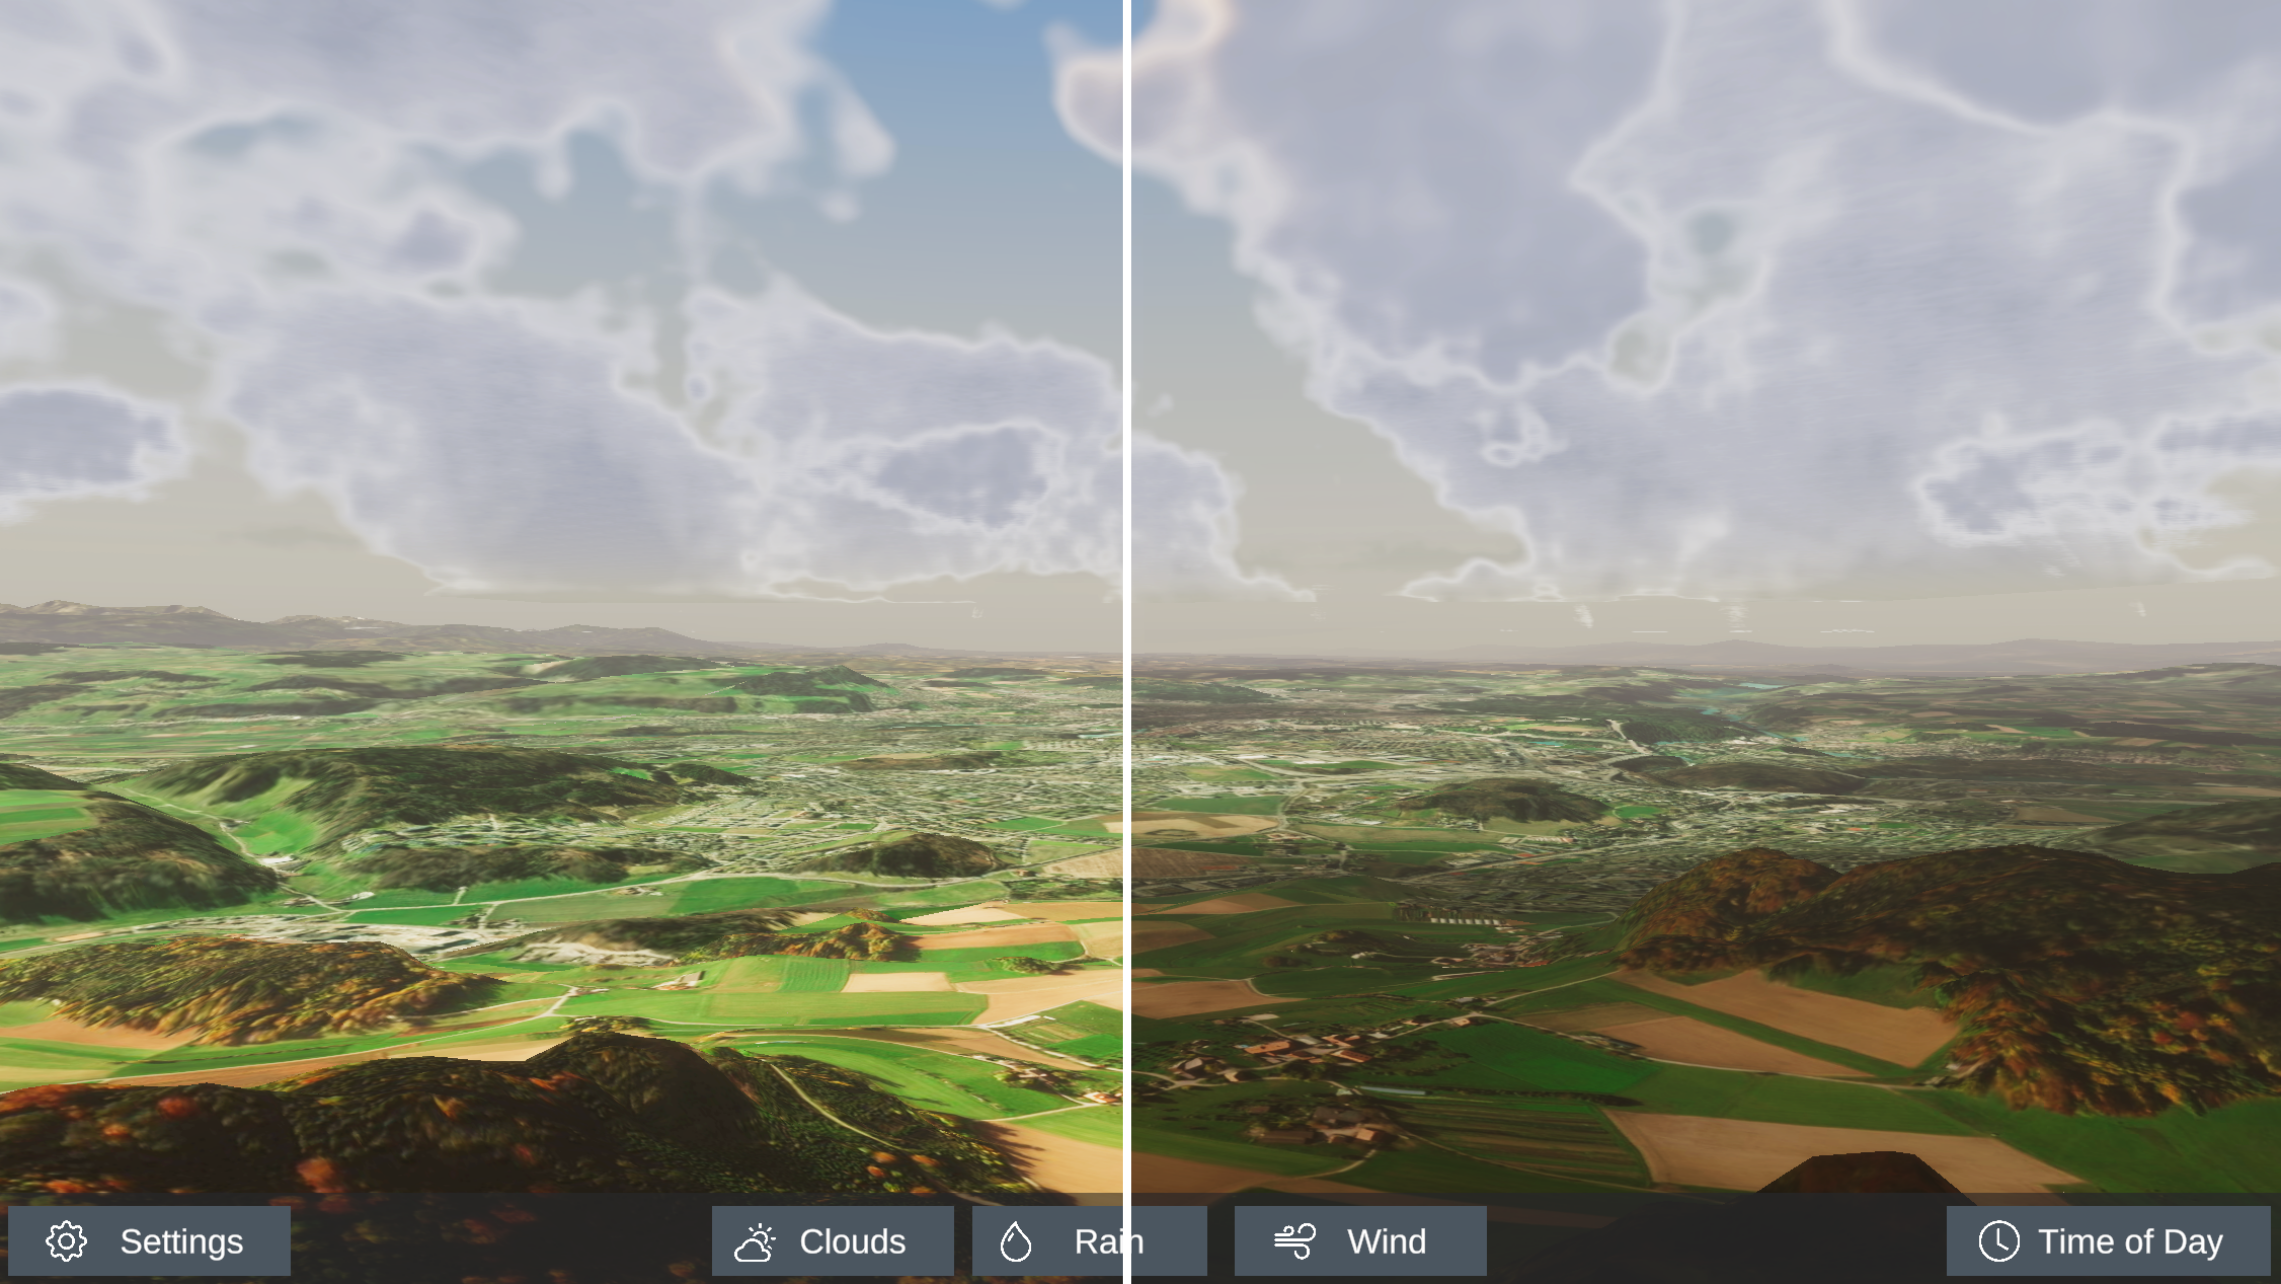
\includegraphics[width=0.8\textwidth]{results/shadow.png}};

        % tile label 1
        \draw (-0.7,4.6) -- (6.9,4.6);
        \draw (-0.7,4.55) -- (-0.7,4.65);
        \draw (6.9,4.55) -- (6.9,4.65);
        \node at (3.1,4.9) {without shadow mapping};
        
        % tile label 2
        \draw (7,-4.4) -- (14.7,-4.4);
        \draw (7,-4.35) -- (7,-4.45);
        \draw (14.7,-4.35) -- (14.7,-4.45);
        \node at (10.85,-4.7) {with shadow mapping};
        
    \end{tikzpicture}
    \captionof{figure}{Visual comparison of a rendered scene with and without the shadow mapping on the ground tiles.}
    \label{img:results:shadowmapping}
\end{figure}

\subsection{Realism and Measurability}
\label{section:techimpl:measure}
% https://diglib.eg.org/xmlui/bitstream/handle/10.2312/EGWR.EGWR01.235-248/235-248.pdf?sequence=1&isAllowed=y

\subsection{Comparison to Previous Work}
\label{section:techimpl:comparison}
